%%%%%%%%%%%%%%%%%%%%%%%%%%%%%%%%%%%%%%%%%%%%%%%%%%%%%%%%%%%%%%%%%%%%%%%%%
%%   CHAPTER: GLIDER SYNTHESIS
%%%%%%%%%%%%%%%%%%%%%%%%%%%%%%%%%%%%%%%%%%%%%%%%%%%%%%%%%%%%%%%%%%%%%%%%%

\renewcommand{\chapterfolder}{glider_synthesis/}
\chapterimage{cover/glider_synthesis}
\chapter{Glider Synthesis}\label{chp:glider_synthesis}\index{glider!synthesis}


\vspace*{-0.4in}
\epigraph{Life isn't about finding yourself. Life is about creating yourself.}{George Bernard Shaw}
\vspace*{0.4in}


\noindent In previous chapters, we saw several different patterns that were capable of generating an endless supply of gliders: glider guns like the Gosper glider gun\index{glider!gun} create streams of gliders coming from a fixed location, and rakes\index{rake} like the space rake create waves of gliders that come from a moving source. We have also seen a few patterns (mostly based on the switch engine\index{switch engine}) capable of creating other objects like blocks or other small still lifes.

In this chapter, we develop a systematic method of constructing patterns that turn these simple objects like gliders and blocks into more complicated objects. In particular, we look at how to collide gliders with each other and with other objects so as to create (or ``synthesize'') new ones. For example, Figure~\ref{fig:lwss_3_gliders} illustrates a method of colliding three gliders so as to produce a lightweight spaceship.

\begin{figure}[!htb]
	\centering\embedlink{lwss_3_gliders}{\vcenteredhbox{\patternimg{0.1}{lwss_3_gliders}} \vcenteredhbox{\genarrow{19}}
		\vcenteredhbox{\patternimg{0.1}{lwss_3_gliders_done}}}
	\caption{Three gliders colliding in such a way as to create a lightweight spaceship.}\label{fig:lwss_3_gliders}
\end{figure}

We call this a \textbf{3-glider synthesis} of the lightweight spaceship, and it is useful because we already know of some patterns (i.e., glider guns) that generate gliders, so we can now create patterns that generate lightweight spaceships: we can just aim the output of three glider guns so as to collide with each other in the right way. For example, Figure~\ref{fig:lwss_gun} uses three Gosper glider guns to create a period~30 lightweight spaceship\index{lightweight!spaceship} gun.

\begin{figure}[!htb]
	\centering\patternimglink{0.1}{lwss_gun}
	\caption{A lightweight spaceship gun constructed by using three Gosper glider guns (top-right, top-left, and bottom-left) to shoot three gliders at each other, which collide in the orientation depicted in Figure~\ref{fig:lwss_3_gliders} in order to create a lightweight spaceship.}\label{fig:lwss_gun}
\end{figure}

There is nothing particularly special about the lightweight spaceship in this example---we will see throughout this chapter that we can collide gliders from glider guns to create a wide variety of moving objects. We can also use gliders to synthesize stationary objects, but for this the glider source has to be moving in order to prevent subsequent gliders from colliding with the synthesized object. Indeed, once we have a large catalog of glider syntheses, the world of Life will open up considerably for us---we will be able to create patterns that construct almost any object in almost any location on the Life plane that we like. 

As one somewhat technical note before we proceed, we require that the gliders in a synthesis could arrive at their positions from arbitrarily far away, since our ultimate goal is to make use of these syntheses via guns and rakes. An example of a glider collision that is \emph{not} considered a true glider synthesis, since there is no way to get the gliders in the indicated positions, is provided in Figure~\ref{fig:invalid_synthesis}.

\begin{figure}[!htb]
	\centering\embedlink{invalid_synthesis}{\vcenteredhbox{\patternimg{0.1}{invalid_synthesis_0}} \vcenteredhbox{\genarrow{22}}
		\vcenteredhbox{\patternimg{0.1}{invalid_synthesis_22}}}
	\caption{A collision of three gliders that produces a block. However, if the two rightmost gliders came from farther away, they would collide with each other before reaching the displayed configuration, so this is not a valid $3$-glider synthesis.}\label{fig:invalid_synthesis}
\end{figure}


\section{Two-Glider Syntheses}\label{sec:2glidersynth}

Once we have a glider synthesis in hand, it is typically straightforward to make use of it, since glider streams can typically be created just by lining up glider guns or rakes in the right spots. But how can we come up with glider syntheses in the first place? For example, how was the three-glider synthesis of a lightweight spaceship in Figure~\ref{fig:lwss_3_gliders} found? The simplest answer, as unsatisfying as it might seem, is to just collide a bunch of gliders together in different ways and catalog which collisions lead to which objects. Once we have a good selection of ``simple'' objects that we know how to synthesize, we can then try colliding gliders with those objects to create more complicated patterns, and so on.

% Ideally one paragraph later
\begingroup\renewcommand{\arraystretch}{0.7}
\begin{table}[!htbp]
	\begin{center}
		\begin{tabular}{Sc Sl Sc Sc Sl}
			\toprule
			Result & 2-Glider Collisions & \qquad \qquad & Result & Collision \\ \midrule
			\specialcell{\embedlink{2_glider_syntheses}{\patternimg{0.162}{block_cropped}} \\ block\index{block}} & \specialcell{\patternlink{2_glider_syntheses}{\patternimg{0.1}{2_glider_block}}} & \qquad \qquad \qquad & \specialcell{\patternlink{2_glider_syntheses}{\patternimg{0.1303902}{boat_cropped}} \\ boat\index{boat}} & \specialcell{\patternlink{2_glider_syntheses}{\patternimg{0.1}{2_glider_boat}}} \\
			
			\rowcolor{gray!20}
			\specialcell{\patternlink{2_glider_syntheses}{\patternimg{0.08763934426}{hf_cropped}} \\ honey farm\index{honey!farm}} & \specialcell{\patternlink{2_glider_syntheses}{\patternimg{0.1}{2_glider_hf}}} & & \specialcell{\patternlink{2_glider_syntheses}{\patternimg{0.10910200408}{beehive_cropped}} \\ beehive\index{beehive}} & \specialcell{\patternlink{2_glider_syntheses}{\patternimg{0.1}{2_glider_beehive}}} \\
			
			\specialcell{\patternlink{2_glider_syntheses}{\patternimg{0.1303902}{blinker_cropped}} \\ blinker\index{blinker}} & \specialcell{\patternlink{2_glider_syntheses}{\patternimg{0.1}{2_glider_blinker}}} & & \specialcell{\patternlink{2_glider_syntheses}{\patternimg{0.10910200408}{loaf_cropped}} \\ loaf\index{loaf}} & \specialcell{\patternlink{2_glider_syntheses}{\patternimg{0.1}{2_glider_loaf}}} \\
			
			\rowcolor{gray!20} \specialcell{\patternlink{2_glider_syntheses}{\patternimg{0.11879996}{tl_cropped}} \\ traffic light\index{traffic light}} & \specialcell{\patternlink{2_glider_syntheses}{\patternimg{0.1}{2_glider_tl}}} & & \specialcell{\patternlink{2_glider_syntheses}{\patternimg{0.11879996}{interchange_cropped}} \\ interchange\index{interchange}} & \specialcell{\patternlink{2_glider_syntheses}{\patternimg{0.1}{2_glider_interchange}}} \\
			
			\specialcell{\patternlink{2_glider_syntheses}{\patternimg{0.1303902}{pi_cropped}} \\ pi-hept.\index{pi-heptomino}\index{pi-heptomino}\index{heptomino!pi|see {pi-heptomino}}} & \specialcell{\patternlink{2_glider_syntheses}{\patternimg{0.1}{2_glider_pi}}} & & \specialcell{\patternlink{2_glider_syntheses}{\patternimg{0.15214731719}{biblock_cropped}} \\ bi-block\index{bi-block}} & \specialcell{\patternlink{2_glider_syntheses}{\patternimg{0.1}{2_glider_biblock}}} \\
			
			\rowcolor{gray!20} \specialcell{\patternlink{2_glider_syntheses}{\patternimg{0.10910200408}{b_cropped}} \\ B-hept.\index{B-heptomino}\index{B-heptomino}} & \specialcell{\patternlink{2_glider_syntheses}{\patternimg{0.1}{2_glider_b}}} & & \specialcell{\patternlink{2_glider_syntheses}{\patternimg{0.10910200408}{eater_1_cropped}} \\ eater 1\index{eater!1}} & \specialcell{\patternlink{2_glider_syntheses}{\patternimg{0.1}{2_glider_eater_1}}} \\
			
			\specialcell{loaf + \\ blinker} & \specialcell{\patternlink{2_glider_syntheses}{\patternimg{0.1}{2_glider_loaf_blinker}}} & & \specialcell{traffic light \\ + glider} & \specialcell{\patternlink{2_glider_syntheses}{\patternimg{0.1}{2_glider_tlg}}} \\
			
			\rowcolor{gray!20} \specialcell{\patternlink{2_glider_syntheses}{\patternimg{0.1303902}{glider_cropped}} \\ glider\index{glider}} & \specialcell{\patternlink{2_glider_syntheses}{\patternimg{0.1}{2_glider_glider}}} & & \specialcell{lumps \\ of muck}\index{lumps of muck} & \specialcell{\patternlink{2_glider_syntheses}{\patternimg{0.1}{2_glider_lom}}} \\
			
			\specialcell{\patternlink{2_glider_syntheses}{\patternimg{0.10910200408}{pond_cropped}} \\ pond\index{pond}} & \specialcell{\patternlink{2_glider_syntheses}{\patternimg{0.1}{2_glider_pond}}} & & \specialcell{\patternlink{2_glider_syntheses}{\patternimg{0.10910200408}{teardrop_cropped}} \\ teardrop\index{teardrop}} & \specialcell{\patternlink{2_glider_syntheses}{\patternimg{0.1}{2_glider_teardrop}}} \\
			
			\rowcolor{gray!20} \specialcell{misc.} & \specialcell{\patternlink{2_glider_syntheses}{\patternimg{0.1}{2_glider_misc}}} & & \specialcell{\patternlink{2_glider_syntheses}{\patternimg{0.10910200408}{octomino_cropped}} \\ octomino} & \specialcell{\patternlink{2_glider_syntheses}{\patternimg{0.1}{2_glider_octomino}}} \\
			
			\specialcell{nothing} & \multicolumn{4}{l}{\specialcell{\\[-0.75em]\patternlink{2_glider_syntheses}{\patternimg{0.1}{2_glider_nothing}}}} \\\bottomrule
		\end{tabular}
		\caption{A summary of the results of all $71$ possible $2$-glider collisions. The four ``misc'' collisions yield somewhat messy combinations of common objects like blocks and blinkers. The rightmost of the ``misc'' collisions (highlighted in \bgbox{redback}{red}) is sometimes called the \textbf{two-glider mess}\index{two-glider mess}, as it takes 530 generations to stabilize---more than any of the other collisions. The left glider-producing collision (highlighted in \bgbox{yellowback2}{yellow}) is called the  \textbf{kickback reaction},\index{kickback reaction} since it produces an output glider traveling in a different direction than either of the input gliders.}\label{tab:2_glider_synth}
	\end{center}
\end{table}
\endgroup

To begin down this road, we look at the simplest type of glider synthesis we can perform: synthesis using a collision of only two gliders. We already saw a few two-glider collisions in Section~\ref{sec:coe_ship} when we aimed two glider waves at each other so as to destroy some gliders and reflect others, and again in Section~\ref{sec:period_catalog} when we aimed two glider waves at each other to create a bi-block wick. Fortunately, cataloging all two-glider syntheses is not too difficult, since there are only 71 different ways that two gliders can collide.\footnote{There does not seem to be a nice ``mathematical'' way to arrive at the number 71 here: it's just a matter of arranging gliders in all possible different orientations and phases and seeing which ones result in collisions.} A full summary of exactly which two-glider collisions lead to which objects being created is provided by Table~\ref{tab:2_glider_synth}.

While the objects that we can create with just two gliders are not particularly exciting, many of them, such as eater~1 and the B-heptomino (which we recall evolves into a Herschel), are essential building blocks of complex patterns. It is also worth pointing out that the two collisions that result in a single glider can in fact sometimes be useful. In particular, the one of these collisions that is on the left in Table~\ref{tab:2_glider_synth} is called the \textbf{kickback reaction}, and it is useful for the fact that the output glider travels in a different direction than either of the two input gliders. This feature can help us navigate gliders around tight spots and simplify many complicated glider syntheses (see Exercise~\ref{exer:glider_synth_two_directions}, for example).


\section{Syntheses Involving Three or More Gliders}\label{sec:3glidersynth}

When moving from two-glider syntheses to three-glider syntheses, things become much more complicated---it is no longer possible to list all collisions and catalog their output, since there are far too many possibilities. To see why this is, recall that the two-glider mess takes 530 generations to stabilize, and we could fire a third glider from dozens of different positions and hundreds of different timings to collide with that chaotic mess. Even worse, that two-glider mess produces multiple gliders, which we could hit with the third glider after an arbitrarily long period of time so as to synthesize a new object as far away as we like.

On the other hand, being unable to catalog all of these three-glider collisions is perhaps not too much of a loss, since we expect that the majority of them would lead to uninteresting combinations of blocks, blinkers, and other common objects that we already know how to synthesize with just two gliders. We thus only present, in Table~\ref{tab:3_glider_synth}, some of the particularly useful three-glider syntheses of more exotic objects. However, we stress that this table is not complete: there are known three-glider syntheses not presented in this table, and it is entirely possible that there are simple objects with three-glider syntheses that have not yet been found.\footnote{For example, the pentadecathlon and switch engine were not known to be synthesizable via only three gliders until the syntheses given in Table~\ref{tab:3_glider_synth} were found by Heinrich Koenig and Luka Okanishi in April 1997 and March 2017, respectively. Similarly, it was not known how to create \emph{any} infinitely growing object using just $3$ gliders until Michael Simkin found a $3$-glider collision that produces a glider-producing switch engine in October 2014.}

\begingroup\renewcommand{\arraystretch}{0.65}
\begin{table}[!htbp]
	\begin{center}		
		\begin{tabular}{Sc Sl}
			\toprule
			Result & 3-Glider Collisions \\\midrule
			\specialcell{\embedlink{tee}{\patternimg{0.135}{glider_cropped}} \\ glider\index{glider}} & \specialcell{\patternlink{tee}{\patternimg{0.1}{3_glider_tee}}} \\
			
			\rowcolor{gray!20} \specialcell{\embedlink{3_glider_lwss}{\patternimg{0.13}{lwss_cropped}} \\ lightweight spaceship\index{lightweight!spaceship}} & \specialcell{\patternlink{3_glider_lwss}{\patternimg{0.1}{3_glider_lwss}}} \\
			
			\specialcell{\embedlink{3_glider_mwss}{\patternimg{0.114}{mwss_cropped}} \\ middleweight spaceship\index{middleweight!spaceship}} & \specialcell{\patternlink{3_glider_mwss}{\patternimg{0.1}{3_glider_mwss}}} \\
			
			\rowcolor{gray!20} \specialcell{\embedlink{3_glider_hwss}{\patternimg{0.101506849315}{hwss_cropped}} \\ heavyweight spaceship\index{heavyweight!spaceship}} & \specialcell{\patternlink{3_glider_hwss}{\patternimg{0.1}{3_glider_hwss}}} \\
			
			\specialcell{\embedlink{3_glider_pentadecathlon}{\patternimg{0.125}{pentadecathlon_cropped}} \\ pentadecathlon\index{pentadecathlon}} & \specialcell{\patternlink{3_glider_pentadecathlon}{\patternimg{0.1}{3_glider_pentadecathlon}}} \\
			
			\rowcolor{gray!20} \specialcell{\embedlink{3_glider_pulsar}{\patternimg{0.13}{pulsar_cropped}} \\ pulsar\index{pulsar}} & \specialcell{\patternlink{3_glider_pulsar}{\patternimg{0.1}{3_glider_pulsar}}} \\
			
			\specialcell{\embedlink{3_glider_queen_bee}{\patternimg{0.11295918367}{queen_bee_cropped}} \\ queen bee\index{queen bee}} & \specialcell{\patternlink{3_glider_queen_bee}{\patternimg{0.1}{3_glider_queen_bee}}} \\
			
			\rowcolor{gray!20} \specialcell{\embedlink{3_glider_r_pentomino}{\patternimg{0.135}{r_pentomino_cropped}} \\ R-pentomino\index{R-pentomino}} & \specialcell{\patternlink{3_glider_r_pentomino}{\patternimg{0.1}{3_glider_r_pentomino}}} \\
			
			\specialcell{\embedlink{3_glider_switch_engine}{\patternimg{0.11}{switch_engine_cropped}} \\ switch engine\index{switch engine}} & \specialcell{\patternlink{3_glider_switch_engine}{\patternimg{0.1}{3_glider_switch_engine}}} \\
			
			\rowcolor{gray!20} \specialcell{glider-producing \\ switch engine \\ (plus junk)\index{glider-producing switch engine}} & \specialcell{\gridbox{0.5pt}{\patternimglink{0.2}{3_glider_switch_engine_glider}}} \\\bottomrule
		\end{tabular}
		\caption{A selection of useful $3$-glider syntheses. The $3$-glider collision that creates a glider-producing switch engine is not a true glider synthesis due to the fact that it also creates a wide assortment of other debris, but it is nonetheless noteworthy for being the only known way of generating infinite growth with just $3$ gliders.}\label{tab:3_glider_synth}
	\end{center}
\end{table}
\endgroup

Although the $3$-glider syntheses of a single glider from Table~\ref{tab:3_glider_synth} (which are called \textbf{tees}\index{tee}) might seem somewhat silly at first glance, they have the useful property that the synthesized glider travels perpendicular to each of the input gliders\footnote{The first two of these syntheses work by colliding two of the gliders so as to create a banana spark\index{banana spark}, which then reflects the third glider as in Figure~\ref{fig:spark_glider_reflect}.}---a property that is not shared by any of its $2$-glider syntheses. For this reason, these syntheses are actually quite useful when trying to manipulate glider positions or reduce the number of directions used in glider syntheses of more complicated objects (see Exercise~\ref{exer:glider_synth_tee}, for example).

The three-glider collision that creates a glider-producing switch engine is quite exciting, as it is our first example of a synthesis of an infinitely growing pattern. Being able to synthesize queen bees is similarly exciting, since a Gosper glider gun is made up of nothing more than two blocks and two queen bees, all of which we now know how to synthesize. By simply synthesizing all of these objects in the correct positions and phases, we are now able to use gliders to synthesize a pattern that creates additional gliders (see Figure~\ref{fig:gosper_glider_synth}),\footnote{Synthesizing the Gosper glider gun ``piece-by-piece'' like this is then quite straightforward, and requires 10 gliders. However, slightly smaller syntheses of the Gosper glider gun are known, requiring as few as 8 gliders.} and we could conceivably use rakes to create Gosper glider guns that in turn create other patterns.

We have a fairly wide variety of objects that we can now synthesize with gliders, but there are still some rather fundamental objects that are missing from our lists of $2$- and $3$-glider syntheses. For example, if we wanted to synthesize a twin bees gun\index{twin bees!gun}, we would first have to know how to synthesize twin bees, which (as far as we know) requires at least $4$~gliders. It is also sometimes beneficial to be aware of glider syntheses that make use of more gliders, even when syntheses involving fewer gliders exist. For example, the $3$-glider synthesis of the heavyweight spaceship given in Table~\ref{tab:3_glider_synth} is actually quite difficult to make use of, since the two gliders coming in from the top-right are so close together that they cannot be generated by many of the glider sources that we have seen (like adjacent Gosper glider guns).

% Ideally 1 paragraph earlier
\begin{figure}[!htb]
	\centering\embedlink{gosper_glider_synth}{\vcenteredhbox{\patternimg{0.1}{gosper_glider_synth_0}} \vcenteredhbox{\genarrow{20}}
		\vcenteredhbox{\patternimg{0.1}{gosper_glider_synth_20}} \vcenteredhbox{\genarrow{20}}
		\vcenteredhbox{\patternimg{0.1}{gosper_glider_synth_40}}}
	\caption{A ten-glider synthesis of a Gosper glider gun, which is composed of two syntheses of blocks (highlighted in \bgbox{aquaback}{aqua}) and two syntheses of queen bees. The queen bee synthesis highlighted in \bgbox{magentaback}{magenta} is the same as the one highlighted in \bgbox{yellowback2}{yellow}, but delayed by 20 generations in order to make the queen bees collide in their proper phases.}\label{fig:gosper_glider_synth}
\end{figure}

For this reason, we often prefer glider syntheses that use widely spaced gliders, even if that comes at the expense of a larger number of gliders. In particular, there are $4$-glider syntheses of a heavyweight spaceship that consist of one glider coming from each direction, and thus are often much easier to make use of. We present a summary of useful syntheses that involve $4$~or more gliders in Table~\ref{tab:other_glider_synth}.

\begin{table}[!htbp]
	\begin{center}
		\begin{tabular}{Sc Sl Sc Sc Sl}
			\toprule
			Result & Glider Syntheses & \qquad \qquad & Result & Synthesis \\ \midrule
			\specialcell{\embedlink{4_glider_clock}{\patternimg{0.125}{clock_cropped}} \\ clock\index{clock}} & \specialcell{\patternlink{4_glider_clock}{\patternimg{0.1}{4_glider_clock}}} & \qquad \qquad \qquad & \specialcell{\embedlink{twin_bees_synth}{\patternimg{0.11}{twin_bees_cropped}} \\ twin bees\index{twin bees}} & \specialcell{\patternlink{twin_bees_synth}{\patternimg{0.1}{twin_bees_synth}}} \\
			
			\rowcolor{gray!20} 
			\specialcell{\embedlink{hwss_4_glider_synth}{\patternimg{0.101506849315}{hwss_cropped}} \\ HWSS\index{heavyweight!spaceship}} & \specialcell{\patternlink{hwss_4_glider_synth}{\patternimg{0.1}{hwss_4_glider_synth}}} & & \specialcell{\embedlink{eater_2_6_gliders}{\patternimg{0.11}{eater_2_cropped}} \\ eater~2\index{eater!2}} & \specialcell{\patternlink{eater_2_6_gliders}{\patternimg{0.1}{eater_2_6_gliders}}} \\\bottomrule
		\end{tabular}
		\caption{Some useful glider syntheses involving $4$ or more gliders. Most of these syntheses have been known for a long time, but the eater~2 synthesis was found by Tanner Jacobi in November 2014 (previously, no synthesis with fewer than $17$ gliders was known, though there were syntheses of slight variants of eater~2 with as few as $8$ gliders).}\label{tab:other_glider_synth}
	\end{center}
\end{table}
% Glider syntheses of spaceships (such as the three-glider syntheses of the lightweight, middleweight, or heavyweight spaceships) can be used to construct guns for these spaceships, as we already saw at the start of this chapter. 


\section{Incremental Syntheses}\label{sec:incremental_synthesis}

Glider syntheses can quickly become cumbersome to use as the number of gliders involved increases. While the guns and rakes that we have already developed let us fire two streams of gliders that collide in any of the 71 possible ways illustrated in Table~\ref{tab:2_glider_synth}, as soon as three or more gliders are involved, it can be quite difficult to coordinate them so that they all arrive at the desired time. For example, it would be challenging to implement the ten-glider synthesis of a Gosper glider gun from Figure~\ref{fig:gosper_glider_synth} ``directly'', as it would require us to coordinate the precise positioning and timing of all ten gliders.

To get around this problem, we make use of \textbf{incremental synthesis}: we build up complicated patterns by first synthesizing a small stable pattern (like a block or a pond), and then collide only a few gliders with that stable pattern to create a slightly more complicated stable pattern, and so on until we arrive at the pattern we actually want. The main benefit of this type of synthesis is that we do not need to be particularly precise with the timing of the gliders---the different stages of synthesis can take place as many generations apart from each other as we like, so we only need to coordinate a few gliders at a time.

As an example, consider the incremental synthesis of the fumarole\index{fumarole} that is presented in Figure~\ref{fig:fumarole_sequential}. While there is a glider synthesis for the fumarole that involves only $7$~gliders (see Exercise~\ref{exer:glider_cleanup}), this $12$-glider synthesis is somewhat easier to make use of, since each stage of its synthesis requires no more than $3$ synchronized gliders.

Incremental syntheses are also advantageous for the fact that we do not have to find ways of synthesizing complicated patterns from scratch, but rather we can keep a catalog of syntheses of various objects, and then to synthesize a new object we can use the most similar still life that we already know how to synthesize as our starting point. For example, the incremental synthesis of the fumarole in Figure~\ref{fig:fumarole_sequential} works by synthesizing a still life that looks similar to the stator of the fumarole (i.e., its stable bottom half), and then the last step of the synthesis creates the fumarole's rotor (i.e., its oscillating top half). This is the most commonly used technique for synthesizing oscillators, and generally billiard table oscillators\index{billiard table} are much more difficult to synthesize than other oscillators precisely because their rotors are contained within their stators and thus this synthesis technique does not work for them.

% Ideally one paragraph earlier
\begin{figure}[!htb]
	\centering\embedlink{fumarole_sequential}{\vcenteredhbox{\patternimg{0.091}{fumarole_sequential_2}} \vcenteredhbox{\gliderarrow{3}} \vcenteredhbox{\patternimg{0.091}{fumarole_sequential_3}} \vcenteredhbox{\gliderarrow{2}} \vcenteredhbox{\patternimg{0.091}{fumarole_sequential_4}} \vcenteredhbox{\gliderarrow{2}} \vcenteredhbox{\patternimg{0.091}{fumarole_sequential_5}} \vcenteredhbox{\gliderarrow{3}} \vcenteredhbox{\patternimg{0.091}{fumarole_sequential_6}}}
	\caption{A $12$-glider incremental synthesis of a fumarole ($2$ gliders that are not shown are required to synthesize the initial beehive). The cells that were created or modified in the previous step of the synthesis are shown in \bgbox{orangeback}{orange}, and the gliders that will be involved in the next collision are shown in \bgbox{greenback}{green}.}\label{fig:fumarole_sequential}
\end{figure}

\begingroup\renewcommand{\arraystretch}{0.7}
\begin{table}[!htbp]
	\begin{center}		
		\begin{tabular}{Sc Sl}
			\toprule
			Result & Last Step of Incremental Synthesis \\\midrule
			\specialcell{\embedlink{tub_sequential}{\patternimg{0.135}{tub_cropped}} \\ tub\index{tub}} & \specialcell{\patternlink{tub_sequential}{\patternimg{0.1}{tub_sequential}}} \\
			
			\rowcolor{gray!20} \specialcell{\embedlink{honey_farm_incremental}{\patternimg{0.08763934426}{hf_cropped}} \\ honey~farm} & \specialcell{\patternlink{honey_farm_incremental}{\patternimg{0.1}{honey_farm_incremental}}} \\
			
			\specialcell{\embedlink{queen_bee_sequential}{\patternimg{0.1}{queen_bee_cropped}} \\ queen~bee\index{queen bee}} & \specialcell{\patternlink{queen_bee_sequential}{\patternimg{0.1}{queen_bee_sequential}}} \\
			
			\rowcolor{gray!20}
			\specialcell{\embedlink{hat_sequential}{\patternimg{0.10910200408}{hat_cropped}} \\ hat\index{hat}} & \specialcell{\patternlink{hat_sequential}{\patternimg{0.1}{hat_sequential}}} \\
			
			\specialcell{\embedlink{ship_sequential}{\patternimg{0.135}{ship_cropped}} \\ ship\index{ship}} & \specialcell{\patternlink{ship_sequential}{\patternimg{0.1}{ship_sequential}}} \\
			
			\rowcolor{gray!20} \specialcell{\embedlink{tub_with_tail_sequential}{\patternimg{0.10910200408}{tub_with_tail_cropped}} \\ tub with tail\index{tub!with tail}} & \specialcell{\patternlink{tub_with_tail_sequential}{\patternimg{0.1}{tub_with_tail_sequential}}} \\
			
			\specialcell{\embedlink{snake_sequential}{\patternimg{0.127}{snake_cropped}} \\ snake\index{snake}} & \specialcell{\patternlink{snake_sequential}{\patternimg{0.1}{snake_sequential}}} \\
			
			\rowcolor{gray!20}
			\specialcell{\embedlink{t_tetromino_incremental}{\patternimg{0.12}{tl_cropped}} \\ T-tetromino / \\ traffic~light\index{T-tetromino}\index{traffic light}} & \specialcell{\patternlink{t_tetromino_incremental}{\patternimg{0.1}{t_tetromino_incremental}}} \\
			
			\specialcell{\embedlink{pentadecathlon_sequential}{\patternimg{0.125}{pentadecathlon_cropped}} \\ pentadecathlon\index{pentadecathlon}} & \specialcell{\patternlink{pentadecathlon_sequential}{\patternimg{0.1}{pentadecathlon_sequential}}} \\
			
			\rowcolor{gray!20} \specialcell{\embedlink{lwss_sequential}{\patternimg{0.11175438596}{lwss_cropped}} \\ LWSS\index{lightweight!spaceship}} & \specialcell{\patternlink{lwss_sequential}{\patternimg{0.1}{lwss_sequential}}} \\
			
			\specialcell{\embedlink{mwss_sequential}{\patternimg{0.09799999999}{mwss_cropped}} \\ MWSS\index{middleweight!spaceship}} & \specialcell{\patternlink{mwss_sequential}{\patternimg{0.1}{mwss_sequential}}} \\
			
			\rowcolor{gray!20} \specialcell{\embedlink{hwss_sequential}{\patternimg{0.087260273972}{hwss_cropped}} \\ HWSS\index{heavyweight!spaceship}} & \specialcell{\patternlink{hwss_sequential}{\patternimg{0.1}{hwss_sequential}}} \\\bottomrule
		\end{tabular}
		\caption{A selection of useful incremental syntheses that can be used to construct many of the simple Life objects that we have seen. Note that the arrangement of a loaf and a blinker in the HWSS incremental synthesis is the exact arrangement produced by the 2-glider syntheses of a loaf and blinker in Table~\ref{tab:2_glider_synth}.}\label{tab:sequential_synth}
	\end{center}
\end{table}
\endgroup

By using the reactions listed in Table~\ref{tab:sequential_synth}, it is straightforward to come up with an incremental synthesis of more complicated objects as well. For example, we can synthesize a Gosper glider gun in a way that never requires more than two synchronized gliders at a time by using incremental syntheses to turn a pond into a ship into a queen bee, as in Figure~\ref{fig:gosper_sequential}. We note that this synthesis uses a total of 12~gliders instead of the 10~gliders used in Figure~\ref{fig:gosper_glider_synth}, but we consider this a small price to pay for the benefit of not having to synchronize as many gliders in any of the steps of synthesis.

Because incremental synthesis typically works by first constructing a still life or a collection of still lifes, and then transforming those still lifes into the desired object, the Life community has gone to great lengths to synthesize still lifes. In fact, syntheses are known for all $190{\thousep}540$ strict still lifes with 20 or fewer live cells.\footnote{It is currently unknown whether or not every strict still life (or every pseudo still life) has a glider synthesis.}

% Ideally 1 paragraph earlier.
\begin{figure}[!htb]
	\centering
	\embedlink{gosper_sequential}{\vcenteredhbox{\patternimg{0.1}{gosper_sequential_0}} \vcenteredhbox{\gliderarrow{4}} \vcenteredhbox{\patternimg{0.1}{gosper_sequential_1}} \vcenteredhbox{\gliderarrow{4}} \vcenteredhbox{\patternimg{0.1}{gosper_sequential_2}} \vcenteredhbox{\gliderarrow{2}} \vcenteredhbox{\patternimg{0.1}{gosper_sequential_3}} \vcenteredhbox{\gliderarrow{2}} \vcenteredhbox{\patternimg{0.1}{gosper_sequential_4}}}
	
	\caption{An incremental synthesis of the Gosper glider gun. Each stage in the synthesis works by either using two gliders to construct a simple still life or using just one glider to transform one object into another one. The objects that were created or modified in the previous step of the synthesis are shown in \bgbox{orangeback}{orange}, and the gliders that will be involved in the next collision are shown in \bgbox{greenback}{green}.}\label{fig:gosper_sequential}
\end{figure}


\section{Synthesis of Moving Objects}\label{sec:incremental_synthesis_ships}

Incremental synthesis is most useful when trying to construct objects that are made up of many simpler objects. We already demonstrated this fact when constructing glider syntheses of the Gosper glider gun, and some other perfect examples include many of the spaceships, puffers, and rakes that we introduced in Chapter~\ref{chp:spaceships}. These objects are mostly composed of many copies of small objects like lightweight spaceships, B-heptominoes, and switch engines that we already know how to synthesize, so we can just synthesize each component individually. However, it can sometimes be tricky to construct the various bits and pieces of these spaceships and puffers with timing that works, so we make these syntheses explicit. 


\subsection{The Ecologist and Space Rake}\label{sec:sequential_space_rake}\index{space rake}

Recall that the ecologist\index{ecologist} of Figure~\ref{fig:ecologist} is made up of three lightweight spaceships and a B-heptomino, so we can synthesize it just by synthesizing those four individual pieces. The only part of the synthesis that is somewhat complicated is the construction of the B-heptomino, since it is not stable without a lightweight spaceship on both sides of it (so we cannot place it first), but there is not enough room for gliders to synthesize it between already-placed lightweight spaceships (so we cannot place it last). One solution is to synthesize the B-heptomino at the same time as the final lightweight spaceship, as in Figure~\ref{fig:ecologist_synth}.

\begin{figure}[!htb]
	\centering
	\embedlink{ecologist_synth}{\vcenteredhbox{\patternimg{0.161}{ecologist_synth0}} \vcenteredhbox{\gliderarrow{3}}
		\vcenteredhbox{\patternimg{0.161}{ecologist_synth1}} \vcenteredhbox{\gliderarrow{3}} \vcenteredhbox{\patternimg{0.161}{ecologist_synth2}} \vcenteredhbox{\gliderarrow{2}} \vcenteredhbox{\patternimg{0.161}{ecologist_synth3}} \vcenteredhbox{\gliderarrow{4}} \vcenteredhbox{\patternimg{0.161}{ecologist_synth4}}}
	\caption{An incremental synthesis of the ecologist. The first two steps simply use one of the three-glider syntheses of lightweight spaceships, and the third step uses a two-glider synthesis of a block. The fourth step is slightly more complicated, since we have to construct the B-heptomino at the same time that we construct the final lightweight spaceship below it. The top two gliders form the B-heptomino, while the bottom two gliders and the block construct a lightweight spaceship via one of the incremental syntheses that we saw in Table~\ref{tab:sequential_synth}.}\label{fig:ecologist_synth}
\end{figure}

There is another way of synthesizing the ecologist that has the advantages of never using more than two synchronized gliders at a time, and only ever using gliders that come from two of the four possible directions. The way that this synthesis works is to first create four lightweight spaceships (three in the positions that we want and one where the B-heptomino should be), each using a two-glider synthesis of a block followed by the two-glider block-to-LWSS synthesis from Table~\ref{tab:sequential_synth}. Then we can fire one additional glider at the central lightweight spaceship to transform it into the desired B-heptomino (to actually get this final glider in the proper orientation though, we make use of the $2$-glider kickback reaction from Table~\ref{tab:2_glider_synth}). The tricky final stage of this synthesis is made explicit in Figure~\ref{fig:ecologist_synth_b}.

Once we have constructed the ecologist, it is straightforward to turn it into the space rake or its backward variant just by synthesizing the extra lightweight spaceship in the correct position, as in Figure~\ref{fig:space_rake_synth} (also see Exercise~\ref{exer:space_rake_synth}). % If desired, this final lightweight spaceship can also be synthesized only using gliders from the same two directions as in the synthesis of the ecologist itself.

\begin{figure}[!htb]
	\centering
	\begin{minipage}[b]{0.43\textwidth}
		\centering
		\embedlink{ecologist_synth_b}{\vcenteredhbox{\patternimg{0.12}{ecologist_synth_b0}} \vcenteredhbox{\genarrow{10}}
			\vcenteredhbox{\patternimg{0.12}{ecologist_synth_b10}} \vcenteredhbox{\genarrow{18}} \vcenteredhbox{\patternimg{0.12}{ecologist_synth_b28}}}
		\caption{Another incremental synthesis of the ecologist. This synthesis has the advantage of never using more than two gliders at a time, and they can all arrive from the lower-left and lower-right (see Exercise~\ref{exer:ecologist_synth}).}\label{fig:ecologist_synth_b}
	\end{minipage}\hfill% The top-left glider looks like it might collide with the lightweight spaceships before getting into the indicated position, but because the lightweight spaceships are moving in the same direction as the glider, they never actually cross paths.
	\begin{minipage}[b]{0.53\textwidth}
		\centering
		\embedlink{space_rake_synth}{\vcenteredhbox{\patternimg{0.12}{space_rake_synth_0}} \vcenteredhbox{\genarrow{8}}
			\vcenteredhbox{\patternimg{0.12}{space_rake_synth_8}} \vcenteredhbox{\genarrow{44}} \vcenteredhbox{\patternimg{0.12}{space_rake_synth_52}}}
		\caption{An incremental glider synthesis of a (forward) space rake. The same technique can be used to synthesize the backward space rake (see Exercise~\ref{exer:space_rake_synth}).}\label{fig:space_rake_synth}
	\end{minipage}
\end{figure}


\subsection{The Schick Engine and Coe Ship}\label{sec:incremental_schick}

To create a glider synthesis of the Schick engine from Section~\ref{sec:schick_engine}, we recall that it is made up of two lightweight spaceships, followed by a spark that is essentially just a T-tetromino\index{T-tetromino} (see Exercise~\ref{exer:six_cell_schick}). The various syntheses of lightweight spaceships and T-tetrominoes that we have seen can thus be used together in a straightforward manner to synthesize the Schick engine, as in Figure~\ref{fig:schick_engine_synth}. The only difficulty comes from having to carefully choose ways of synthesizing the individual components so that they do not interfere with each other.

\begin{figure}[!htb]
	\centering
	\embedlink{schick_engine_synth}{\vcenteredhbox{\patternimg{0.1}{schick_engine_synth_0}} \vcenteredhbox{\gliderarrow{4}}
		\vcenteredhbox{\patternimg{0.1}{schick_engine_synth_3}} \vcenteredhbox{\genarrow{26}} \vcenteredhbox{\patternimg{0.1}{schick_engine_synth_26}}}
	\caption{A glider synthesis of a Schick engine. Lightweight spaceships are created by the \bgbox{magentaback}{magenta} and \bgbox{aquaback}{aqua} glider collisions, and a T-tetromino (which becomes the Schick engine's trailing spark) is created by the gliders outlined in \bgbox{yellowback2}{yellow}.}\label{fig:schick_engine_synth}
\end{figure}

With this synthesis of the Schick engine in hand, we are also now able to synthesize the period~$60$ variants of the space rake that we saw in Section~\ref{sec:schick_engine}---we just synthesize the space rake and then synthesize a Schick engine next to it in the appropriate position, or vice-versa (see Exercise~\ref{exer:make_space_rake_synth}(b)).

Synthesizing the Coe ship is slightly less straightforward, since we have not yet seen how to synthesize the deformed heavyweight spaceship that makes up half of it. Perhaps the simplest way to synthesize this object is to first synthesize a lightweight and middleweight spaceship next to each other, and then use two additional gliders to transform the MWSS into the deformed HWSS, as illustrated in Figure~\ref{fig:coe_ship_synth}.

\begin{figure}[!htb]
	\centering
	\embedlink{coe_ship_incremental}{\vcenteredhbox{\patternimg{0.12}{coe_ship_synth_0}} \vcenteredhbox{\gliderarrow{4}} \vcenteredhbox{\patternimg{0.12}{coe_ship_synth_1}} \vcenteredhbox{\gliderarrow{2}} \vcenteredhbox{\patternimg{0.12}{coe_ship_synth_2}}}
	\caption{An incremental glider synthesis of a Coe ship that works by synthesizing a lightweight spaceship next to a middleweight spaceship, and then transforming that middleweight spaceship into the necessary deformed heavyweight spaceship.}\label{fig:coe_ship_synth}
\end{figure}


% https://conwaylife.com/forums/viewtopic.php?f=&p=41558#p41557
\subsection{Corderships}\label{sec:cordership_synth}\index{Cordership}

Corderships make up another family of objects that are prime candidates for glider synthesis, since they are also made up of several easily synthesized components---switch engines.\index{switch engine} The difficult part of synthesizing a Cordership is that the switch engines have to be synchronized with each other, making an incremental synthesis difficult. Since each switch engine requires at least three gliders to synthesize, we expect the $10$-engine Cordership from Figure~\ref{fig:10_engine_cordership} to require at least $30$ gliders to synthesize. Furthermore, the $6$ front and middle switch engines will have to be constructed at almost the exact same time as each other.\footnote{Despite these obstacles, Stephen Silver created a $60$-glider synthesis of the $10$-engine Cordership in 1998 (using a 4-glider synthesis of a switch engine, since the 3-glider synthesis was not yet known).}

With these difficulties in mind, it seems desirable to try synthesizing a Cordership that uses as few switch engines as possible---the $2$-engine Cordership from Exercise~\ref{exer:2_engine_cordership} or the $3$-engine Cordership from Exercise~\ref{exer:3_engine_cordership}. Here we focus on the $3$-engine Cordership, and we leave the task of synthesizing its $2$-engine counterpart to Exercise~\ref{exer:2_engine_cordership_synthesis}.

As expected, it is not too difficult to use $3 \times 3 = 9$ gliders to synthesize the three switch engines that make up this Cordership. However, one small problem arises after we use these $9$~gliders: while the Cordership is indeed synthesized correctly, the switch engines take a few generations to sync up with each other, so some unwanted debris is left behind. To prevent this debris from forming, we use $2$~extra gliders---one for each of the outermost switch engines---to suppress some chaotic reactions that are normally suppressed by the central switch engine. Altogether, this results in the $11$-glider synthesis of the $3$-engine Cordership displayed in Figure~\ref{fig:3_engine_cordership_synthesis}.

\begin{figure}[!htb]
	\centering
	\embedlink{3_engine_cordership_synthesis}{\vcenteredhbox{\phantom{$\cdots$ \genarrow{71}}} \vcenteredhbox{\patternimg{0.1}{3_engine_cordership_synthesis_0}} \vcenteredhbox{\fixarrowc{47}} \vcenteredhbox{\patternimg{0.1}{3_engine_cordership_synthesis_47}}} \\[1em]
	
	\patternlink{3_engine_cordership_synthesis}{\vcenteredhbox{$\cdots$ \genarrow{71}} \vcenteredhbox{\patternimg{0.1}{3_engine_cordership_synthesis_118}} \vcenteredhbox{\genarrow{232}} \vcenteredhbox{\patternimg{0.1}{3_engine_cordership_synthesis_350}}} \\[1em]
	\caption{An $11$-glider synthesis of the $3$-engine Cordership. The $3$~switch engines are synthesized by the $3$-glider syntheses highlighted in \bgbox{aquaback}{aqua}, \bgbox{magentaback}{magenta}, and \bgbox{greenpastel}{green}. The remaining $2$~gliders clean up some extra junk that would otherwise be left behind by the outermost switch engines.}\label{fig:3_engine_cordership_synthesis}
\end{figure}



\section{Developing New Syntheses}\label{sec:new_syntheses}

So far the glider syntheses that we have seen have been restricted to two basic types: (a)~syntheses that were found just by crashing gliders together and cataloging what objects were created, and (b)~syntheses that can be made simply by piecing together the syntheses of type~(a). We now branch out and demonstrate how to construct glider syntheses of more exotic objects that do not decompose in any natural way into simpler objects that we already know how to synthesize.

Perhaps the most common way to develop new glider syntheses is to find a soup\index{soup} that leaves behind the pattern of interest in its ash, and try to reverse-engineer the part of the soup's evolution that led to the object's formation. To illustrate this method, consider Rich's p16\index{Rich's p16} (the period~16 oscillator that we introduced in Figure~\ref{fig:rich_p16}), which was found by evolving the soup displayed in Figure~\ref{fig:richs_p16_soup}.

\begin{figure}[!ht]
	\centering\embedlink{richs_p16_soup}{\vcenteredhbox{\patternimg{0.1464}{richs_p16_soup}} \vcenteredhbox{\genarrow{196}} \vcenteredhbox{\patternimg{0.11}{richs_p16_soup_196}}}
	\caption{The soup that led to the discovery of Rich's p16 (highlighted on the right in \bgbox{aquaback}{aqua}).}\label{fig:richs_p16_soup}
\end{figure}

To develop a glider synthesis for this oscillator, we evolve the soup to just before its formation (in this case, slightly earlier than generation $196$) and try to isolate the reaction that creates the oscillator. In this step, it is important to keep in mind that the goal is to go back far enough that all (or at least most) of the reactions are ones that we are familiar with, such as a T-tetromino or a queen bee colliding with some still lifes. In this particular case, if we go to generation $164$ of the soup's evolution then the reaction has decomposed enough that we can identify all of the important pieces of the oscillator's creation: Rich's p16 (plus a lot of extra debris) forms when two honey farm predecessors and two B-heptominoes collide in a specific way with two blocks and two beehives (see Figure~\ref{fig:richs_p16_soup_detailed}).

\begin{figure}[!htb]
	\centering
	\begin{subfigure}{.48\textwidth}
		\centering\patternlink{richs_p16_soup}{\patternimg{0.13}{richs_p16_soup_164}}
		\caption{Generation~164.}\label{fig:richs_p16_soup_164}
	\end{subfigure} \ \ \ \ % 
	\begin{subfigure}{.48\textwidth}
		\centering\patternlink{richs_p16_soup}{\patternimg{0.13}{richs_p16_soup_155}}
		\caption{Generation~155.}
		\label{fig:richs_p16_soup_155}
	\end{subfigure}
	\caption{Rich's p16 is created (a) when two honey farm predecessors (highlighted in \bgbox{yellowback2}{yellow}) and two B-heptominoes (highlighted in \bgbox{greenpastel}{green}) collide with two blocks and two beehives (highlighted in \bgbox{magentaback}{magenta}). The honey farm predecessors can be identified by comparing them with Figure~\ref{fig:pre_honeyfarm}, and the B-heptomino can be identified by (b) going backward to generation~155 of the soup.}\label{fig:richs_p16_soup_detailed}
\end{figure}

We now have enough tools at our disposal to synthesize this oscillator, since we know how to synthesize blocks, beehives, honey farms, and B-heptominoes. However, the B-heptominoes in this reaction are quite messy, and create a lot of leftover debris that we would then have to clean up with several additional gliders (see Exercise~\ref{exer:single_glider_cleanup}). To reduce the number of required gliders somewhat, we notice that only three cells on one side of the B-heptominoes interact with the rest of the reaction, and only for two generations. Another easy-to-synthesize object with the same configuration of three cells is the eater~1, which can thus replace the B-heptominoes as in Figure~\ref{fig:richs_p16_predecessor}. Fortunately, using eater~1s in this way does result in a much smaller amount of debris being created around Rich's p16.

\begin{figure}[!ht]
	\centering\embedlink{richs_p16_predecessor}{\vcenteredhbox{\patternimg{0.11}{richs_p16_predecessor}} \vcenteredhbox{\genarrow{32}} \vcenteredhbox{\patternimg{0.11}{richs_p16_predecessor_32}}}
	\caption{A reaction of common objects that results in Rich's p16 (and two unwanted boats). This is the same reaction as in Figure~\ref{fig:richs_p16_soup_164}, but with the B-heptominoes replaced by eater~1s (highlighted in \bgbox{greenpastel}{green}).}\label{fig:richs_p16_predecessor}
\end{figure}

The only somewhat tricky part of synthesizing this collection of objects is creating the two honey farm predecessors, since they are unstable and we thus have to create them after creating the still lifes. For this reason, we opt to use the incremental honey farm synthesis from Table~\ref{tab:sequential_synth}, so that instead of having to use $4$ coordinated gliders in the final stage of synthesis ($2$ for each honey farm), we only need to use $2$ coordinated gliders (plus $2$ blocks that we can place much earlier). A complete incremental synthesis of this oscillator is presented in Figure~\ref{fig:richs_p16_synthesis}.\footnote{This synthesis was originally found by Charlie Neder, using the method we outlined in this section, and posted to the ConwayLife.com forums less than a day after the oscillator's discovery.} We stress that there is nothing particularly clever about this synthesis; it just makes use of the $2$-glider syntheses from Table~\ref{tab:2_glider_synth}, the incremental honey farm synthesis we already mentioned, and one final glider collision (which is easily found by hand) to destroy the left-over boats.

\begin{figure}[!ht]
	\centering
	\embedlink{richs_p16_synthesis}{\vcenteredhbox{\patternimg{0.179}{richs_p16_synthesis_1}} \vcenteredhbox{\gliderarrow{4}} \vcenteredhbox{\patternimg{0.179}{richs_p16_synthesis_2}} \vcenteredhbox{\gliderarrow{4}} \vcenteredhbox{\patternimg{0.179}{richs_p16_synthesis_3}} \vcenteredhbox{\gliderarrow{6}} \vcenteredhbox{\patternimg{0.179}{richs_p16_synthesis_4}} \vcenteredhbox{\gliderarrow{2}} \vcenteredhbox{\patternimg{0.179}{richs_p16_synthesis_5}} \vcenteredhbox{\gliderarrow{2}} \vcenteredhbox{\patternimg{0.179}{richs_p16_synthesis_6}}}
	
	\caption{An $18$-glider incremental synthesis of Rich's p16. The first three stages of synthesis just involve placing still lifes that can each be synthesized by $2$ gliders. The next stage synthesizes the honey farm predecessors, and the final stage uses $2$ additional gliders to destroy the $2$ leftover boats. Objects that were created or modified in the previous step of the synthesis are shown in \bgbox{orangeback}{orange}, and the gliders that will be involved in the next collision are shown in \bgbox{greenback}{green}.}\label{fig:richs_p16_synthesis}
\end{figure}


\section{A Gosper Glider Gun Breeder}\label{sec:gosper_breeder}

We have now learned quite a few recipes for synthesizing different objects with gliders. To demonstrate how useful these glider syntheses can be, we now switch focus a bit and start \emph{using} these glider syntheses to create new types of patterns. In particular, we now construct our first \textbf{breeder}\index{breeder}: an object that grows quadratically (as opposed to objects like guns or rakes, which grow linearly). In other words, we will construct an object that does not just fill up some \emph{strip} of the Life plane, but instead fills an ever-expanding \emph{region} of the Life plane.

The idea behind this breeder is simple enough: we use the rakes that we introduced in Section~\ref{sec:rakes} to fire gliders in such a way that those gliders synthesize Gosper glider guns (using the incremental synthesis from Figure~\ref{fig:gosper_sequential}). Since the rakes will create Gosper glider guns at a linear rate, and the Gosper glider guns will then each create gliders at a linear rate, the overall growth of our pattern will be quadratic.

% Ideally 2 paragraphs later
\begin{figure}[!htb]
	\centering
	\patternimglinkwidth{\textwidth}{breeder_front}
	\caption{The front end of our breeder features two copies of the period~60 backward space rake (outlined in \bgbox{yellowback2}{yellow}), followed by two copies of the period~60 forward space rake (outlined in \bgbox{aquaback}{aqua}), all traveling to the right. The gliders from these rakes collide in such a way as to create ponds, which is the first step of the incremental synthesis of a Gosper glider gun presented in Figure~\ref{fig:gosper_sequential}.}\label{fig:breeder_front}
\end{figure}

To make this construction explicit, we first note that we cannot possibly use the period~20 space rakes directly, since they can only be used to construct objects that are 10~cells apart. Since Gosper glider guns are wider than that, they would collide and destroy each other. We thus make use of the slightly more complicated period~60 variants of the space rake that we introduced in Section~\ref{sec:schick_engine}, which will produce glider guns that are 30~cells apart from each other.

Now we just go through the Gosper glider gun's incremental synthesis step by step, lining up rakes so that the gliders they produce collide in the desired way. For example, for the first step of the synthesis (i.e., creating the two initial ponds), we need four rakes, which we can position as in Figure~\ref{fig:breeder_front}.

Once we have positioned those four rakes, they create two endless lines of ponds with a distance of 30~cells between each consecutive pair. At this point, we simply move on to the next portion of the glider synthesis: we construct two blocks near each pair of ponds, which we can do with four more rakes. We then need to hit the ponds with a single glider each in order to turn them into ships, which we do with two more rakes. Lastly, we use two final rakes to fire gliders at the pair of ships, turning each of them into queen bees and thus completing the Gosper glider gun synthesis. The resulting breeder is displayed in Figure~\ref{fig:breeder_done}.\footnote{The first breeder was found by Bill Gosper in the early 1970s. It used the exact same ideas that we used in the construction of our breeder, but used a different puffer in place of the space rakes that we used.}

\begin{figure}[!ht]
	\centering
	\patternimglinkwidth{\textwidth}{breeder_done}
	\caption{A breeder constructed using an incremental glider synthesis of a Gosper glider gun. First, on each side, a forward and a backward p60 space rake collaborate to create a pond as in Figure~\ref{fig:breeder_front} (outlined on the right in \bgbox{yellowback2}{yellow}), followed by another paired forward and backward space rake creating a block (outlined in \bgbox{greenpastel}{green}). Next, a backward space rake converts the pond into a ship (outlined in \bgbox{aquaback}{aqua}), and finally another backward space rake converts the ship into a queen bee (outlined in \bgbox{magentaback}{magenta}), thus completing the synthesis of the Gosper glider gun.}\label{fig:breeder_done}
\end{figure}

In generation~0 (i.e., its starting phase), this breeder has a population of $2038$ cells. The quadratic growth of this breeder can be quantified by noting that every 60~generations, an additional $44$-cell Gosper glider gun is created, and each of those guns creates two additional $5$-cell gliders, for a total population in generation $60n$ of $5n^2 + 44n + 2038$. This quadratic growth is illustrated in Figure~\ref{fig:breeder_done_1200}, which shows the expanding triangular region of gliders behind generation~1200 of the breeder.

\begin{figure}[!htb]
	\centering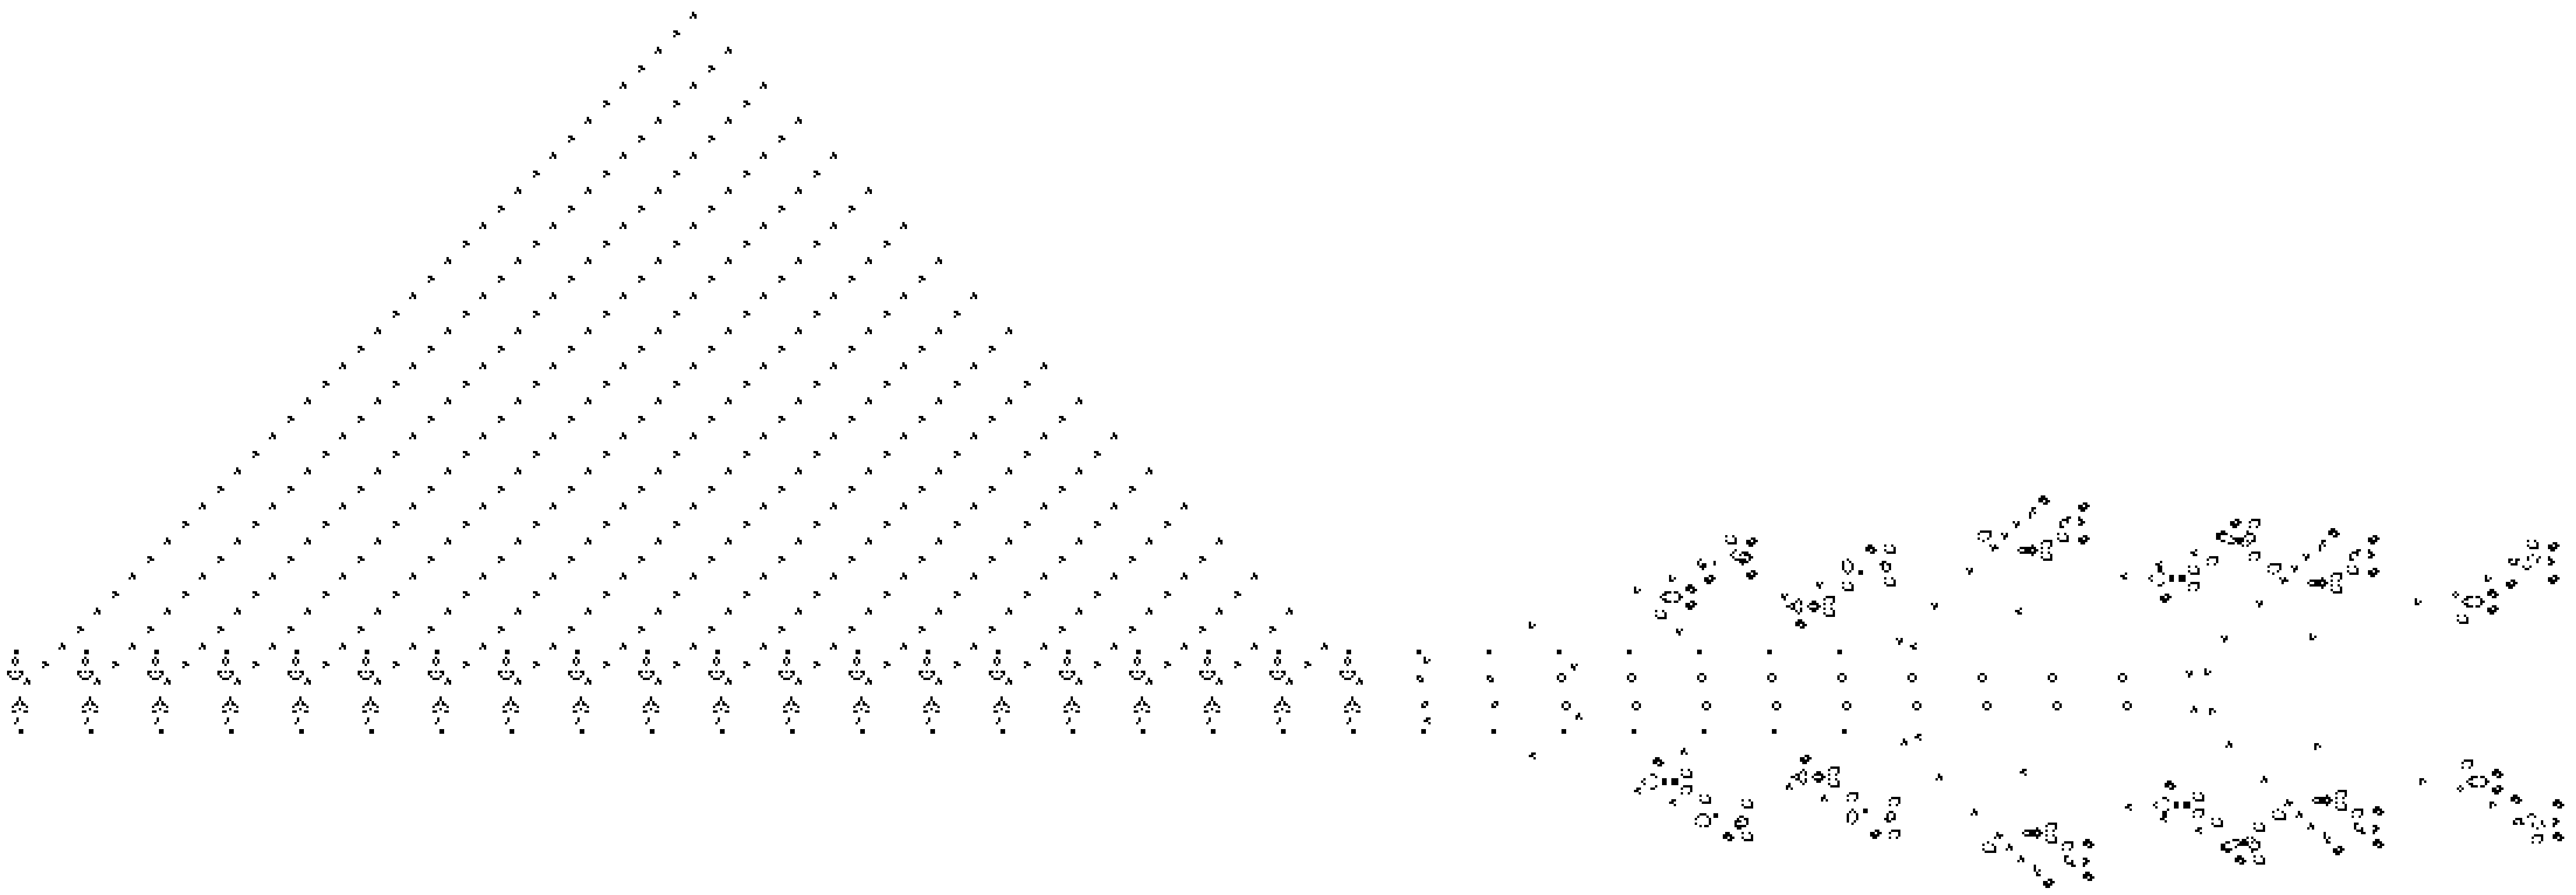
\includegraphics[width=\textwidth]{glider_synthesis/breeder_done_1200.png}
	\caption{After running the breeder for 1200~generations, we see a triangle of gliders form at the west, above the line of Gosper glider guns that has been synthesized. As the breeder moves farther to the east, the triangle continues to expand to the northeast.}\label{fig:breeder_done_1200}
\end{figure}

While this breeder is quite large, we have purposely not optimized it, in order to make the mechanisms that make it work more apparent. The space rakes can be moved much closer to each other without compromising its functionality (see Exercise~\ref{exer:breeder_minimize}), and by cleverly manipulating the space rake debris it is actually possible to place more than one of the still lifes at the same time, thus halving the total number of space rakes from $12$ to $6$. We present and make use of a much more compact Gosper glider gun breeder that comes from these ideas a bit later, in Section~\ref{sec:primer_itself}.



\section{Slow Salvo Synthesis}\label{sec:slow_salvo}

In Section~\ref{sec:incremental_synthesis}, we saw that we can often break glider syntheses down into bits and pieces that are individually easy to understand and make use of. In this section, we take this idea to its most extreme by considering \textbf{slow salvos}\index{salvo}, which are collections of gliders\footnote{Technically, a salvo can be made up of any spaceships, but the term almost always refers to gliders.} that (a) are \textbf{slow}: only one glider interacts in the synthesis at a time, and (b) form a \textbf{salvo}: all of the gliders come from the same direction.

In order for the gliders in a slow salvo to be able to actually synthesize anything, we need another object (called a \textbf{seed}\index{seed}) for it to crash into. While we could in principle use any object, it is typical to use a block\index{block} as a starting point, since it is the simplest and most symmetric stationary object. Furthermore, it is typical to only consider either \textbf{p1 slow salvos} or \textbf{p2 slow salvos}, which are slow salvos in which the intermediate objects that are created after every glider collision are still lifes or some combination of still lifes and period~2 oscillators, respectively.\footnote{P2 salvos are advantageous because blinkers are so easy to synthesize, and we will see shortly that the clock\index{clock} is also a useful tool when working with slow salvos. We could analogously consider p$n$ slow salvos for some $n \geq 3$, but in practice not much is gained by doing so, since objects with period~3 or higher typically aren't any easier to create in intermediate stages of synthesis than objects of period~1 or period~2.} This perhaps seems like quite an extensive list of restrictions, but we have in fact already seen a few objects that can be created via p1 slow salvos. For example, we saw in Table~\ref{tab:sequential_synth} that we could use a pond as a seed in a p1~slow salvo to produce a ship, and then a queen bee.% As a less trivial example, consider the p1 slow salvo synthesis presented in Figure~??, which uses a total of 12 gliders to gradually change the starting block into more and more complicated still lifes, eventually resulting in an eater~1. Compare this synthesis with the one presented in Figure~\ref{fig:17_cell_synthesis}, which was neither slow (multiple gliders are involved in most stages of synthesis) nor a salvo (gliders approach from all four directions).

Despite how restrictive slow salvos seem at first, it is a remarkable fact that they are exactly as general as standard glider syntheses. That is, if we can synthesize an object with gliders at all then we can synthesize it with a p2 slow salvo.\footnote{However, the slow salvo might contain considerably more gliders than other glider syntheses.} In order to pin down exactly why this is the case, we now introduce several new reactions that allow us to systematically create slow salvo syntheses from standard glider syntheses.


\subsection{Creating and Moving Blocks}\label{sec:slow_salvo_blocks}

Our first step toward showing that slow salvos can construct anything that regular glider syntheses can is to demonstrate how we can create almost any arrangement of any number of blocks in the Life plane that we like. The first reaction that we will need is the one displayed in Figure~\ref{fig:slow_salvo_splitter}, which uses a slow salvo of $2$ gliders to turn a single block into two blocks.

\begin{figure}[!htb]
	\centering\embedlink{slow_salvo_splitter}{\vcenteredhbox{\patternimg{0.101}{slow_salvo_splitter_0}} \vcenteredhbox{\gliderarrow{1}} \vcenteredhbox{\patternimg{0.101}{slow_salvo_splitter_1}} \vcenteredhbox{\gliderarrow{1}} \vcenteredhbox{\patternimg{0.101}{slow_salvo_splitter_2}}}
	\caption{A $2$-glider slow salvo can turn one block into two blocks.}\label{fig:slow_salvo_splitter}
\end{figure}

While the two resulting blocks are in very different positions than the initial block, it turns out that this does not particularly matter, as we can also use p1 slow salvos to move a block from one position on the Life plane to any other. To show that such a movement is possible, we use the two block-moving reactions displayed in Figure~\ref{fig:block_movers}. The first of these reactions uses a single glider to move a block up $2$~cells and left $1$~cell (in fact, this is exactly the (2,1) block pull\index{(2,1) block pull} that we saw way back in Figure~\ref{fig:glider_block_move}), and the second reaction uses six gliders (in a p1 slow salvo) to move a block down and to the right $1$ cell.

If we repeat these two reactions, then we can move a block a single cell up, down, left, or right. For example, to move a block up a single cell, we could perform the movement in Figure~\ref{fig:block_move_1_glider}, followed by the movement in Figure~\ref{fig:block_move_6_gliders} (for a total cost of $7$ gliders). Similarly:\smallskip

\begin{itemize}
	\item To move a block right by a single cell, we could perform the movement in Figure~\ref{fig:block_move_1_glider}, followed by the movement in Figure~\ref{fig:block_move_6_gliders} twice.\footnote{This requires a total of $13$ gliders, which is far from optimal---another p1 slow salvo is known that accomplishes the same movement via only $7$~total gliders. However, we are just interested in presenting the conceptually simplest method of moving blocks, not necessarily the most efficient one. Paul Chapman and Dave Greene put together an extensive table of the cheapest known block-moving slow salvos, which is available at \httpurl{b3s23life.blogspot.com/2004/09/glues-slow-salvo-block-move-table.html} (note that the values in their table assume that the gliders come from the bottom-right, rather than the top-left).}\smallskip
	
	\item To move a block left by a single cell, we could perform the movement in Figure~\ref{fig:block_move_1_glider}, but reflected along the diagonal from the top-left to the bottom right. Then perform the movement in Figure~\ref{fig:block_move_6_gliders}.\smallskip
	
	\item To move a block down by a single cell, we could first move it left by a single cell and then perform the movement in Figure~\ref{fig:block_move_6_gliders}.\smallskip
\end{itemize}

% Ideally 1 paragraph before the bullet list above.
\begin{figure}[!htb]
	\centering
	\begin{tabular}{@{}cc@{}}
		\begin{subfigure}[b]{.39\textwidth}
			\centering\embedlink{block_move_1_glider}{\vcenteredhbox{\patternimg{0.176}{block_move_1_glider_0}} \vcenteredhbox{\gliderarrow{1}} \vcenteredhbox{\patternimg{0.176}{block_move_1_glider_1}}}
			\caption{The (2,1) block pull is a reaction in which a single glider pulls a block by $2$~cells in one direction and $1$~cell in the other.}\label{fig:block_move_1_glider}
		\end{subfigure} &
		\begin{subfigure}[b]{.59\textwidth}
			\centering\raisebox{-0.48\height}{\begin{tikzpicture}[scale=0.5, every node/.style={transform shape}]%
				\node[inner sep=0pt,anchor=south west] at (0,0) {\embedlink{block_move_6_gliders}{\patternimg{0.2}{block_move_6_gliders_0}}};
				
				\colorletternode{green}{5.8}{2.85}{1}
				\colorletternode{green}{4.7}{4.6}{2}
				\colorletternode{green}{5.8}{6.3}{3}
				\colorletternode{green}{2.3}{2.85}{4}
				\colorletternode{green}{1.65}{4.6}{5}
				\colorletternode{green}{0.3}{5.6}{6}
				\end{tikzpicture}} \patternlink{block_move_6_gliders}{\vcenteredhbox{\gliderarrow{6}} \vcenteredhbox{\patternimg{0.1}{block_move_6_gliders_6}}}
			\caption{A $6$-glider slow salvo moving a block down and right by $1$ cell.}\label{fig:block_move_6_gliders}
		\end{subfigure}
	\end{tabular}
	\caption{Two methods of moving a block around with p1 slow salvos. The order in which the gliders should come in is indicated by the \bgbox{greenpastel}{green} numbers---their exact timing does not matter, as long as they are far enough apart that each collision settles down before the next glider arrives. Repeating these slow salvos allows us to move a block to any position on the Life plane.}
	\label{fig:block_movers}
\end{figure}

Now that we know how to use p1 slow salvos to move a block by a single cell in any direction, we can easily repeat these reactions over and over until the block is moved to whatever position we desire. However, there are a few other block-moving slow salvos that are worth making note of, since they help us move blocks around the plane a bit more quickly. In particular, if we are willing to make use of p2 salvos instead of just p1 ones, then we gain access to the salvos displayed in Figure~\ref{fig:p2_block_movers}. There are hundreds of salvos of this type known.\footnote{A collection of them is available at \httpsurl{conwaylife.com/forums/viewtopic.php?p=8182\#p8182}.} It is worth noting that the \textbf{(2,1) block push}\index{(2,1) block push} of Figure~\ref{fig:block_push_2_1} \emph{pushes} the block by the same amount that the $(2,1)$ block pull of Figure~\ref{fig:block_move_1_glider} pulls it.

% General note now about pushes being more expensive than pulls?

\begin{figure}[!htb]
	\centering
	\begin{tabular}{@{}cccc@{}}
		\begin{subfigure}[b]{.205\textwidth}
			\centering
			\raisebox{-0.48\height}{\begin{tikzpicture}[scale=0.5, every node/.style={transform shape}]%
				\node[inner sep=0pt,anchor=south west] at (0,0) {\embedlink{block_push_2_1}{\patternimg{0.1850615094}{block_push_2_1}}};
				
				\colorletternode{green}{3.97}{2.7}{1}
				\colorletternode{green}{2}{1.5}{2}
				\colorletternode{green}{2.4}{3.3}{3}
				\colorletternode{green}{0.4}{4.55}{4}
				\colorletternode{green}{3.95}{6.15}{5}
				\end{tikzpicture}}
			\caption{$(2,1)$ block push.}\label{fig:block_push_2_1}
		\end{subfigure} &
		\begin{subfigure}[b]{.21\textwidth}
			\centering
			\raisebox{-0.48\height}{\begin{tikzpicture}[scale=0.5, every node/.style={transform shape}]%
				\node[inner sep=0pt,anchor=south west] at (0,0) {\embedlink{block_move_1_neg1}{\patternimg{0.1850615094}{block_move_1_neg1}}};
				
				\colorletternode{green}{3.9}{2.75}{1}
				\colorletternode{green}{2.35}{1.15}{2}
				\colorletternode{green}{2.05}{3.65}{3}
				\colorletternode{green}{0.5}{2.1}{4}
				\colorletternode{green}{2.3}{5.7}{5}
				\colorletternode{green}{0.5}{6.2}{6}
				\end{tikzpicture}}
			\caption{$(1,-1)$ block move.}\label{fig:block_move_1_neg1}
		\end{subfigure} &
		\begin{subfigure}[b]{.27\textwidth}
			\centering
			\raisebox{-0.48\height}{\begin{tikzpicture}[scale=0.5, every node/.style={transform shape}]%
				\node[inner sep=0pt,anchor=south west] at (0,0) {\embedlink{block_move_11_0}{\patternimg{0.2541}{block_move_11_0}}};
				
				\colorletternode{green}{6.3}{3.3}{1}
				\colorletternode{green}{4.25}{5.35}{2}
				\colorletternode{green}{0.68}{3.82}{3}
				\colorletternode{green}{1.25}{5.72}{4}
				\end{tikzpicture}}
			\caption{$(11,0)$ block pull.\index{(11,0) block pull}}\label{fig:block_move_11_0}
		\end{subfigure} &
		\begin{subfigure}[b]{.23\textwidth}
			\centering
			\raisebox{-0.48\height}{\begin{tikzpicture}[scale=0.5, every node/.style={transform shape}]%
				\node[inner sep=0pt,anchor=south west] at (0,0) {\embedlink{block_push_11_0}{\patternimg{0.15089630767}{block_push_11_0}}};
				
				\colorletternode{green}{3.45}{4.9}{1}
				\colorletternode{green}{2.15}{6.2}{2}
				\colorletternode{green}{2.65}{2.25}{3}
				\colorletternode{green}{1.85}{3.75}{4}
				\colorletternode{green}{0.35}{5.05}{5}
				\colorletternode{green}{4.65}{6.35}{6}
				\end{tikzpicture}}
			\caption{$(11,0)$ block push.\index{(11,0) block push}}\label{fig:block_push_11_0}
		\end{subfigure}
	\end{tabular}
	\caption{Some p2 slow salvos that move a block by various amounts. The output location of the block is highlighted in \bgbox{greenpastel}{green}.}
	\label{fig:p2_block_movers}
\end{figure} 


% IMPORTANT http://conwaylife.com/forums/viewtopic.php?f=2&t=918&p=7291&hilit=blockic#p7291
\subsection{One-Time Turners}\label{sec:slow_salvo_turners}

Just like we can use gliders to create and move blocks around the Life plane, we can also use blocks to move gliders around the Life plane. We can thus use a p1 slow salvo to create arrangements of blocks that then change the direction of other gliders in the salvo, thus creating salvos that come from multiple directions.

To be a bit more explicit, consider the arrangement of blocks presented in Figure~\ref{fig:one_time_turner}, which can be used to rotate a glider by 90 degrees, but is destroyed in the process (contrast this with reflectors like the Snark\index{Snark}, which rotate gliders but remain unchanged). Reflectors like this are called \textbf{one-time turners}\index{one-time turner}, and they are one of the key ingredients that let us emulate arbitrary glider syntheses via slow salvos. There are also numerous other 90-degree one-time turners involving various numbers of blocks (and sometimes other small still lifes---see Exercise~\ref{exer:boat_one_time_turner}), but this turner involving just two blocks is perhaps the simplest, and for now it is enough for our purposes.

\begin{figure}[!htb]
	\centering\embedlink{one_time_turner}{\vcenteredhbox{\patternimg{0.14}{one_time_turner_0}} \vcenteredhbox{\genarrow{35}} \vcenteredhbox{\patternimg{0.14}{one_time_turner_35}}}
	\caption{A \textbf{one-time turner} composed of two blocks that rotates a glider by 90 degrees and destroys the blocks at the same time.}\label{fig:one_time_turner}
\end{figure}

Importantly, because this one-time turner is made up of nothing other than blocks, we can construct it using a p1 slow salvo via the techniques that we developed in the previous section. An explicit $12$-glider p1 slow salvo that does the job (and also leaves us with an extra block that we can then use to construct additional turners) is displayed in Figure~\ref{fig:create_one_time_turner}. This salvo works by using 2 gliders to duplicate the initial block (as in Figure~\ref{fig:slow_salvo_splitter}), 8 gliders to move one of these blocks to a new position, and then 2 more gliders to duplicate this block again.% (and due to the clever way we repositioned the second block, this second duplication leaves a pair of blocks in exactly the one-time turner configuration).

\begin{figure}[!htb]
	\centering\raisebox{-0.5\height}{\begin{tikzpicture}[scale=0.518, every node/.style={transform shape}]%
		\node[inner sep=0pt,anchor=south west] at (0,-0.2) {\embedlink{create_one_time_turner}{\patternimg{0.195}{create_one_time_turner_0}}};
		
		\colorletternode{green}{4.2}{3.75}{1}
		\colorletternode{green}{4.15}{5.9}{2}
		\end{tikzpicture}} \patternlink{create_one_time_turner}{\vcenteredhbox{\gliderarrow{2}}} \raisebox{-0.5\height}{\begin{tikzpicture}[scale=0.518, every node/.style={transform shape}]%
		\node[inner sep=0pt,anchor=south west] at (0,-0.2) {\patternlink{create_one_time_turner}{\patternimg{0.195}{create_one_time_turner_2}}};
		
		\colorletternode{green}{3.07}{6.35}{1}
		\colorletternode{green}{1.69}{7}{2}
		\colorletternode{green}{2.15}{5}{3}
		\colorletternode{green}{1.47}{5.87}{4}
		\colorletternode{green}{0.61}{6.74}{5}
		\colorletternode{green}{0.15}{7.87}{6}
		\colorletternode{green}{1.73}{8.09}{7}
		\colorletternode{green}{1.02}{8.98}{8}
		\end{tikzpicture}} \patternlink{create_one_time_turner}{\vcenteredhbox{\gliderarrow{8}}} \raisebox{-0.5\height}{\begin{tikzpicture}[scale=0.518, every node/.style={transform shape}]%
		\node[inner sep=0pt,anchor=south west] at (0,-0.2) {\patternlink{create_one_time_turner}{\patternimg{0.195}{create_one_time_turner_10}}};
		
		\colorletternode{green}{5.05}{4.8}{1}
		\colorletternode{green}{5}{7}{2}
		\end{tikzpicture}} \patternlink{create_one_time_turner}{\vcenteredhbox{\gliderarrow{2}}} \raisebox{-0.5\height}{\begin{tikzpicture}[scale=0.518, every node/.style={transform shape}]%
		\node[inner sep=0pt,anchor=south west] at (0,-0.2) {\patternlink{create_one_time_turner}{\patternimg{0.195}{create_one_time_turner_12}}};
		\end{tikzpicture}}
	\caption{A 12-glider p1 slow salvo creating the one-time turner from Figure~\ref{fig:one_time_turner} (highlighted in \bgbox{magentaback}{magenta}) and leaving behind another block to create additional turners or other objects with. The first $2$ gliders duplicate the initial block via the reaction of Figure~\ref{fig:slow_salvo_splitter}, the next $8$ gliders move one of the blocks down and to the right, and then the final $2$ gliders duplicate that moved block.}% The order in which the gliders should come in is indicated by the \bgbox{greenpastel}{green} numbers---their exact timing does not matter, as long as they are far enough apart that each collision settles down before the next glider arrives.}
	\label{fig:create_one_time_turner}
\end{figure}

We can thus use a total of $13$ gliders in a p1 slow salvo ($12$~to create the one-time turner and $1$~to use and destroy it) to create $1$~glider in a perpendicular direction, while still having a block left over to perform additional constructions with. Using this technique, we are now able to emulate multi-directional glider syntheses via unidirectional syntheses.

For example, consider the four-glider syntheses of the clock\index{clock} that we saw in Table~\ref{tab:other_glider_synth}, which each use one glider coming from all four possible directions. A unidirectional synthesis of the clock can be constructed by using a p1 slow salvo to construct four one-time turners---one of the gliders does not need to be turned at all, two gliders need to be turned once each, and one glider needs to be turned twice---and then firing four gliders at the one-time turners with the proper timing. An explicit configuration of one-time turners that works is displayed in Figure~\ref{fig:unidirection_clock_synthesis}.\footnote{It is possible to create a p1 slow salvo that builds this arrangement of blocks by hand, but there are also computer scripts that automate this process---see Exercise~\ref{exer:create_clock_turners}.}

\begin{figure}[!htb]
	\centering\embedlink{unidirection_clock_synthesis}{\vcenteredhbox{\patternimg{0.1}{unidirection_clock_synthesis}} \vcenteredhbox{\genarrow{135}} \vcenteredhbox{\patternimg{0.1}{unidirection_clock_synthesis_135}}}
	\caption{One-time turners (which can be synthesized with a p1 slow salvo) can be used to allow unidirectional glider waves (like the one on the left) to emulate multi-directional glider syntheses (like the one on the right). The gliders on the right are in exactly the position of the clock synthesis that we saw in Table~\ref{tab:other_glider_synth}.}\label{fig:unidirection_clock_synthesis}
\end{figure}


\clearpage% for layout reasons


Unfortunately, this construction does not give us a true p1 slow salvo for constructing a clock, since the final four gliders in the synthesis (i.e., the ones that hit the one-time turners) must be synchronized with each other---we are not free to space them arbitrarily far from one another. In order to fix this problem, we need to introduce some methods for using blocks to duplicate gliders and adjust their timing.


% http://conwaylife.com/forums/viewtopic.php?f=2&t=1512
% table of blockic splitters: http://conwaylife.com/forums/viewtopic.php?f=2&t=1065#p7661
\subsection{Splitters and Timing}\label{sec:slow_salvo_splitters}

The first ingredient that we need in order avoid having to send synchronized gliders at our one-time turners is a method of turning one glider into many gliders. Just like our one-time turner, we would like this pattern to be composed entirely of blocks, and we would like it to be cleanly destroyed during the glider-duplicating reaction. Patterns with these properties are called \textbf{blockic splitters}\index{blockic splitter},\footnote{The term \textbf{blockic} refers to the fact that it is composed entirely of blocks. There are also splitters (and one-time turners) made up of other still lifes (or even blinkers), but we do not consider them here since blocks are enough for our purposes.} and one example is provided in Figure~\ref{fig:one_time_splitter}.

\begin{figure}[!htb]
	\centering\embedlink{one_time_splitter}{\vcenteredhbox{\patternimg{0.15}{one_time_splitter_0}} \vcenteredhbox{\genarrow{202}} \vcenteredhbox{\patternimg{0.09}{one_time_splitter_202}}}
	\caption{A \textbf{blockic splitter}, which uses three blocks to turn one glider into four gliders (while destroying the blocks in the process).}\label{fig:one_time_splitter}
\end{figure}

This splitter \emph{almost} gets us what we need---it lets us turn one glider into four, and we could chain multiple splitters together to turn one glider into as many as we desire. We can use one-time turners to move these gliders around the Life plane, with the intention of emulating multi-direction glider syntheses, but unfortunately we are faced with two brand new problems:\smallskip

\begin{itemize}
	\item The one-time turner that we introduced in Figure~\ref{fig:one_time_turner} preserves the glider's color,\index{glider!color} so we have no way of obtaining glider color combinations other than those provided to us by the splitter in Figure~\ref{fig:one_time_splitter} (in which the bottom-left glider has the same color as the input glider, and the other $3$ gliders have the opposite color). Since the $4$-glider synthesis of a clock uses $2$ gliders of each color, in order to make a slow salvo synthesis of the clock we would have to use this splitter multiple times and then use blocks to delete the excess gliders, which is quite wasteful.\smallskip
	
	\item The one-time turner from Figure~\ref{fig:one_time_turner} gives us no control over timing, and we need some way of making sure that all of the desired gliders in a given synthesis not only arrive at the right place, but also at the right time.\smallskip
\end{itemize}

Fortunately, there is a common solution to both of the above problems, and it is simply to introduce several new one-time turners. In particular, the numerous 180-degree one-time turners presented in Table~\ref{tab:180_degree_one_time_turners} are capable of either preserving or changing the color of a glider, and also offsetting its timing by any amount that we desire.%\footnote{This collection of 180-degree one-time turners was compiled by Dave Greene.}

\begin{table}[!ht]\vspace*{0.05in}
	\begin{center}		
		\begin{tabular}{Sc Sc Sc Sc Sc Sc Sc}
			\toprule
			& \multicolumn{4}{c}{Delay} \\  \cmidrule{2-5}
			& $0$ & $1$ & $2$ & $3$ \\ \midrule
			\specialcell{Color-\\ Preserving} & \specialcell{\embedlink{180_degree_one_time_turners}{\patternimg{0.12}{180_one_time_turner_0_0}}} & \specialcell{\patternlink{180_degree_one_time_turners}{\patternimg{0.12}{180_one_time_turner_0_1}}} & \specialcell{\patternlink{180_degree_one_time_turners}{\patternimg{0.12}{180_one_time_turner_0_2}}} & \specialcell{\patternlink{180_degree_one_time_turners}{\patternimg{0.12}{180_one_time_turner_0_3}}} \\
			\specialcell{Color-\\ Changing} & \specialcell{\patternlink{180_degree_one_time_turners}{\patternimg{0.12}{180_one_time_turner_1_0}}} & \specialcell{\patternlink{180_degree_one_time_turners}{\patternimg{0.12}{180_one_time_turner_1_1}}} & \specialcell{\patternlink{180_degree_one_time_turners}{\patternimg{0.12}{180_one_time_turner_1_2}}} & \specialcell{\patternlink{180_degree_one_time_turners}{\patternimg{0.12}{180_one_time_turner_1_3}}} \\\cmidrule{2-5}
			& $4$ & $5$ & $6$ & $7$ \\\cmidrule{2-5}
			\specialcell{Color-\\ Preserving} & \specialcell{\patternlink{180_degree_one_time_turners}{\patternimg{0.12}{180_one_time_turner_0_4}}} & \specialcell{\patternlink{180_degree_one_time_turners}{\patternimg{0.12}{180_one_time_turner_0_5}}} & \specialcell{\patternlink{180_degree_one_time_turners}{\patternimg{0.12}{180_one_time_turner_0_6}}} & \specialcell{\patternlink{180_degree_one_time_turners}{\patternimg{0.12}{180_one_time_turner_0_7}}} \\
			\specialcell{Color-\\ Changing} & \specialcell{\patternlink{180_degree_one_time_turners}{\patternimg{0.12}{180_one_time_turner_1_4}}} & \specialcell{\patternlink{180_degree_one_time_turners}{\patternimg{0.12}{180_one_time_turner_1_5}}} & \specialcell{\patternlink{180_degree_one_time_turners}{\patternimg{0.12}{180_one_time_turner_1_6}}} & \specialcell{\patternlink{180_degree_one_time_turners}{\patternimg{0.12}{180_one_time_turner_1_7}}} \\\bottomrule
		\end{tabular}
		\caption{By using different 90-degree one-time turners together, we can create this collection of 180-degree one-time turners that lets us set a glider to any timing and color. In all cases, the input glider is highlighted in \bgbox{greenback}{green} and comes in from the top-left, while the location of the output glider exactly 200 generations later is highlighted in \bgbox{orangeback}{orange}. The boats are not required for the turners to function, but just serve to make it easier to line up multiple different turners.}\label{tab:180_degree_one_time_turners}
	\end{center}
\end{table}


\clearpage% for layout reasons


In order to make use of these 180-degree one-time turners to put gliders in (almost) any \emph{position} that we want, we first simply use copies of the 90-degree one-time turner from Figure~\ref{fig:one_time_turner} and the 180-degree one-time turners with offset~0 from Table~\ref{tab:180_degree_one_time_turners}. Importantly, we always place at least one 180-degree turner in the path of each glider, even if it is not required to get its positioning right (we will need that 180-degree turner to get the timing right momentarily).

Even though the positioning of the gliders is now correct, their timing will likely be horribly wrong. To fix this problem, we now focus on the glider that gets to its destination last---we will synchronize all of the other gliders with this one. To slow down those other gliders, we note that moving a 180-degree turner $1$ cell farther away causes the glider to reach its destination $8$ generations later (it now has to travel $1$ cell, and thus $4$ generations, farther in both directions). To delay a glider by $n$ generations, we can thus move its 180-degree turner farther away by $\lfloor n/8 \rfloor$ generations and then replace it by the turner from Table~\ref{tab:180_degree_one_time_turners} that has the same effect on its color but has offset $n \ \text{mod} \ 8$.

We now have a complete set of glider-preserving or glider-changing turners capable of delaying a glider by any of $0,1,2,\ldots,7$ generations.  So we have all the tools we need to position \emph{and} time gliders as we see fit. An example of how we can use the $4$ gliders produced by the splitter in Figure~\ref{fig:one_time_splitter} to synthesize a clock is presented in Figure~\ref{fig:clock_slow_salvo}. Note that we placed a 180-degree one-time turner in the path of each of the four gliders so that we could use the technique for correcting their timing described in the previous paragraph, and since each of those 180-degree turners is simply made up of two 90-degree one-time turners, we are able to separate their two halves in order to more easily control the glider's output position.

\begin{figure}[!htb]
	\centering
	\patternimglinkwidth{\textwidth}{clock_slow_salvo}
	\caption{A \textbf{blockic seed} for a clock: The blockic splitter at the top-center (highlighted in \bgbox{orangeback2}{orange}) turns the single incoming glider into four gliders whose paths are outlined in \bgbox{yellowback2}{yellow}, \bgbox{greenpastel}{green}, \bgbox{aquaback}{aqua}, and \bgbox{magentaback}{magenta}. Those gliders are repeatedly reflected via one-time turners in such a way that they end up in the indicated positions required to synthesize a clock after $537$ generations. We could probably get away with using fewer one-time turners, but by placing a 180-degree turner in the path of every glider it is much easier to get their timing right.}
	\label{fig:clock_slow_salvo}
\end{figure}

A configuration of simple still lifes, like the one in Figure~\ref{fig:clock_slow_salvo}, that synthesizes a particular object when hit by a glider (or gliders) is called a \textbf{seed}\index{seed} (and a seed made up entirely of blocks is called a \textbf{blockic seed}).\index{blockic seed} Seeds are particularly useful since they immediately give us a p1 slow salvo for constructing an object---a clock in this case---since we ``just'' have to use a p1 slow salvo to construct the still lifes in the seed and then fire one additional glider to trigger the synthesis.

However, actually building a slow salvo synthesis for a seed is a tedious process. The $31$-block seed for a clock from Figure~\ref{fig:clock_slow_salvo} requires hundreds of slow gliders to construct (see Exercise~\ref{exer:create_clock_turners_nonsync})---recall that we already needed 12 gliders just to create a single $2$-block one-time turner in Figure~\ref{fig:create_one_time_turner}. For this reason, slow salvo syntheses of seeds are typically built by computer scripts, with \emph{slsparse}\index{slsparse}\index{slmake|see {slsparse}} (see \httpsurl{conwaylife.com/wiki/Slsparse} for tutorials and a download link) being the most widely used.% Even very small syntheses can require hundreds or thousands of gliders to emulate in a p1 slow salvo.\footnote{As an example, Dave Greene constructed an explicit p1 slow salvo consisting of 997 gliders that constructs a configuration of 81 blocks that, when hit by one additional glider, transforms into an 8-glider synthesis of the loafer\index{loafer} spaceship. This salvo can be seen at \httpsurl{conwaylife.com/forums/viewtopic.php?f=2\&t=1006\&p=7574\#p7574}.}


\subsection{Tight Packings of Gliders}\label{sec:slow_salvo_tight}

There is still one final problem that might arise when trying to emulate an arbitrary glider synthesis via a slow salvo synthesis, and that is the fact that some syntheses involve packings of gliders coming from the same direction that are too close together for us to place with our one-time turners. This was not a problem for the clock synthesis in Figure~\ref{fig:clock_slow_salvo} since each of the gliders in the synthesis comes from a different direction. However, if we were to try to use a p1 slow salvo to emulate the 3-glider synthesis of an HWSS displayed in Table~\ref{tab:3_glider_synth}, it is not obvious that we can position the two gliders that are heading southwest close enough to each other (since one of the gliders might interfere with any one-time turner that we try to use to position the other glider). To fix this glider-packing problem, we introduce one final reaction: the \textbf{clock inserter}\index{clock!inserter},\footnote{Found by Martin Grant in December 2014.} which uses two opposing gliders to transform a clock\index{clock} into a perpendicular glider, as in Figure~\ref{fig:clock_inserter}.

\begin{figure}[!htb]
	\centering
	\embedlink{clock_inserter}{\vcenteredhbox{\phantom{$\cdots$ \genarrow{1}}} \vcenteredhbox{\patternimg{0.1}{clock_inserter_0}} \vcenteredhbox{\genarrow{1}} \vcenteredhbox{\patternimg{0.1}{clock_inserter_1}} \vcenteredhbox{\genarrow{1}} \vcenteredhbox{\patternimg{0.1}{clock_inserter_2}} \vcenteredhbox{\genarrow{1}} \vcenteredhbox{\patternimg{0.1}{clock_inserter_3}} \vcenteredhbox{\phantomarrowa{} $\cdots$} \\[1em]
		\vcenteredhbox{$\cdots$ \genarrow{1}} \vcenteredhbox{\patternimg{0.1}{clock_inserter_4}} \vcenteredhbox{\genarrow{1}} \vcenteredhbox{\patternimg{0.1}{clock_inserter_5}} \vcenteredhbox{\genarrow{1}} \vcenteredhbox{\patternimg{0.1}{clock_inserter_6}} \vcenteredhbox{\genarrow{1}} \vcenteredhbox{\patternimg{0.1}{clock_inserter_7}} \vcenteredhbox{\phantom{\phantomarrowa{} $\cdots$}}}
	\caption{The \textbf{clock inserter} is a reaction that very cleanly collides two gliders in such a way as to transform a clock into a perpendicular glider. The two-glider collision produces a domino spark in generation~5 (shown in \bgbox{orangeback}{orange}) and then dies off, while the domino spark\index{domino spark} initiates the clock-to-glider transformation. The debris at the bottom-right in generation~8 dies off in 5 more generations.}\label{fig:clock_inserter}
\end{figure}

The key facts that make this reaction so useful for us are (1) that the output glider appears at a small offset and moves through the space just vacated by the colliding input gliders, and (2) the reaction is almost effortless---it does not disrupt any other cells around the clock and output glider, and thus does not disrupt other nearby gliders either. This reaction can thus be used to place a glider very close in front of, or to the side of, another already-placed glider (see Figure~\ref{fig:clock_inserter_effective} for an illustration of how closely it can place a new glider to other gliders). Because of this, we can use this reaction to build any arrangement of gliders, no matter how tight, as long as we start by placing the gliders in the back first. Actually \emph{proving} that the clock inserter reaction can be used to build any arrangement of gliders is somewhat technical and messy,\footnote{Chris Cain wrote a script that automatically uses clock inserters to build glider arrangements in 2014, and then he and Dave Greene used the script to build such a wide array of tight glider arrangements that this could probably be considered the first proof that p2 slow salvos can build any configuration of gliders. Cain's script can be found at \httpsurl{conwaylife.com/forums/viewtopic.php?p=15133\#p15133}.} since there are many possible ways for gliders to be near each other, so we defer the proof to Appendix~\ref{chp:appendix_salvo}.

With this reaction in hand, we can now use a p2 slow salvo to construct any arrangement of gliders in the plane that we desire. First, we ``rewind'' the desired glider synthesis back as far as we like, so that it consists of four salvos of gliders---one coming from each direction.\footnote{Recall that the gliders must be able to reach their positions from arbitrarily far away in order to be considered a valid glider synthesis.} We then construct the four salvos one glider at a time. If the gliders in a salvo are spaced sufficiently far apart, we can insert gliders into it via one-time turners. If the gliders are spaced close together, we instead first synthesize a clock (via p1 slow salvo synthesis, such as in Figure~\ref{fig:clock_slow_salvo}) and then use the clock inserter to insert the close gliders one at a time. We have thus finally proved the following theorem:

\begin{theorem}[Universality of p2 Slow Salvo Synthesis]\label{thm:p2_slow_salvo}
	Every pattern that can be constructed via glider synthesis can be constructed by a p2 slow salvo glider synthesis.
\end{theorem}

\begin{figure}[!htb]
	\centering
	\embedlink{clock_inserter_effective}{\vcenteredhbox{\patternimg{0.115}{clock_inserter_effective_0}} \vcenteredhbox{\genarrow{52}} \vcenteredhbox{\patternimg{0.115}{clock_inserter_effective_52}}}
	\caption{A demonstration of how the clock inserter (shown in \bgbox{greenback}{green} on the left) can be used to place a glider (shown in \bgbox{orangeback}{orange} on the right) closely beside and in front of other already-placed gliders.}\label{fig:clock_inserter_effective}
\end{figure}

The only p2 object that we needed to prove Theorem~\ref{thm:p2_slow_salvo} was the clock, which we used to place clusters of tightly packed gliders. We can get around having to use clocks (and thus avoid p$2$ objects altogether) by instead using the blockic seed of a clock from Figure~\ref{fig:clock_slow_salvo}. More specifically, if we wish to use a clock insertion reaction, we first split a single glider into three via blockic splitters---one of those gliders then hits the seed, creating a clock, and the other two are reflected so as to trigger the clock insertion reaction as in Figure~\ref{fig:clock_inserter}. Since this entire process is carried out by a single glider in the slow salvo synthesis, the result is a p1 slow salvo synthesis. We thus have the following strengthening of Theorem~\ref{thm:p2_slow_salvo}:\footnote{There are some mild technicalities that we have glossed over here---see Exercise~\ref{exer:p2_salvo_reduce_to_p1}.}%\footnote{The fact that some p2 clocks are created during this synthesis is irrelevant, since they are destroyed before the next glider in the salvo arrives.}

\begin{theorem}[Universality of p1 Slow Salvo Synthesis]\label{thm:p1_slow_salvo}
	Every pattern that can be constructed via glider synthesis can be constructed by a p1 slow salvo glider synthesis.
\end{theorem}


% http://conwaylife.com/forums/viewtopic.php?f=2&t=1512&start=25#p23670
% IMPORTANT: http://conwaylife.com/forums/viewtopic.php?f=2&t=1006&p=7574#p7574
%% Last 15-bit SL: http://conwaylife.com/forums/viewtopic.php?f=2&t=1155&start=75#p9258
%% Last 16-bit SL: http://conwaylife.com/forums/viewtopic.php?f=2&t=1155&start=225#p10227
%% Last 17-bit SL: http://conwaylife.com/forums/viewtopic.php?f=2&t=1276&start=100#p11972
%% Last 18-bit SL: http://conwaylife.com/forums/viewtopic.php?f=2&t=1467&start=50#p14272
%% 5-glider very long snake: http://conwaylife.com/forums/viewtopic.php?f=2&t=1452&p=17219#p17102
%%%%%%%%%%%%%%%%%%%%%%%%%%%%%%%%
\section{Notes and Historical Remarks}\label{sec:synthesis_notes}
%%%%%%%%%%%%%%%%%%%%%%%%%%%%%%%%

The importance of glider synthesis was known essentially as soon as the glider itself was found in 1970, with common folklore being that we could send gliders as signals throughout the Life plane and collide those gliders in different ways to simulate arbitrary computations. This basic idea has been refined and made more precise repeatedly over the past 50 years, to the point that there are now explicit patterns that do exactly this---they collide gliders so as to perform arbitrary computations and build almost any pattern of our choosing (we will delve deeply into the specifics of how these patterns work in Chapters~\ref{chp:universal_computation} and~\ref{chp:universal_construction}).

The first specific and explicit uses of glider syntheses were demonstrated in 1971, when Bill Gosper constructed the first breeder (essentially the breeder that we built in Section~\ref{sec:gosper_breeder}) as well as the first lightweight and middleweight spaceship guns. These patterns demonstrated the kind of leap in complexity that is possible when taking advantage of glider synthesis, and it led to a surge in interest in the topic over the following years.

By 1973, the majority of ``basic'' Life objects were synthesizable, including lightweight, middleweight, and heavyweight spaceships, switch engines (and their block-laying and glider-producing counterparts), commonly occurring oscillators like the pentadecathlon and pulsar, and all still lifes and oscillators with 7 or fewer cells other than the clock and the long snake. Syntheses of larger composite patterns were even being discovered by this point, with Douglas Petrie constructing the $11$-glider synthesis of the Schick engine displayed in Figure~\ref{fig:schick_engine_synth} in 1973. The majority of these early syntheses were developed by David Buckingham, Mark Niemiec, and Douglas Petrie.

Over the following decades, David Buckingham continued to develop syntheses for still lifes and oscillators, and he completed syntheses of all of them with $14$ or fewer cells by no later than 1992. His technique was to make heavy use of incremental synthesis, building the objects from the inside out, only using a couple of gliders at a time to tweak the outermost portion of the object that he was synthesizing. This method works very well when synthesizing objects that have ``end pieces'' like tails that can be removed or altered without affecting the pattern's stability. However, compact still lifes like the one in Figure~\ref{fig:14_cell_synth} are much more difficult to construct, and this particular still life (which was the last $14$-cell still life to be synthesized) was initially synthesized using a massive incremental synthesis involving more than $30$ gliders.

\begin{figure}[!htb]
	\centering
	\begin{subfigure}{.135\textwidth}
		\centering\patternimglink{0.135}{14_cell_synth}
		\caption{$14$ cells.}\label{fig:14_cell_synth}
	\end{subfigure} \ \ \ \ % 
	\begin{subfigure}{.135\textwidth}
		\centering\patternimglink{0.135}{15_cell_synth}
		\caption{$15$ cells.}\label{fig:15_cell_synth}
	\end{subfigure} \ \ \ \ % 
	\begin{subfigure}{.13\textwidth}
		\centering\patternimglink{0.135}{16_cell_synth}
		\caption{$16$ cells.}\label{fig:16_cell_synth}
	\end{subfigure} \ \ \ \ % 
	\begin{subfigure}{.14\textwidth}
		\centering\patternimglink{0.135}{17_cell_synth}
		\caption{$17$ cells.}\label{fig:17_cell_synth}
	\end{subfigure} \ \ \ \ % 
	\begin{subfigure}{.14\textwidth}
		\centering\patternimglink{0.135}{18_cell_synth}
		\caption{$18$ cells.}\label{fig:18_cell_synth}
	\end{subfigure} \ \ \ \ % 
	\begin{subfigure}{.145\textwidth}
		\centering\patternimglink{0.12161157024}{19_cell_synth}
		\caption{$19$ cells.}\label{fig:19_cell_synth}
	\end{subfigure}
	\caption{The final still lifes with $14$--$19$ cells to be synthesized by gliders.}\label{fig:hard_to_synth_sls}
\end{figure}

Mark Niemiec continued on with this work, creating a large database that he used to automatically generate syntheses of thousands of still lifes by piecing together known reactions \cite{Nie03,Nie10}. This greatly reduced the number of still life syntheses that needed to be found by hand, and in 2013 he, with help from Martin Grant, completed syntheses of all $15$-cell still lifes (as well as syntheses for all except for a few hundred 16-, 17-, and 18-cell still lifes).

% ideally 2 paragraphs later
\begin{figure}[!htb]
	\centering
	\embedlink{17_cell_synthesis}{\vcenteredhbox{\phantom{$\cdots$ \gliderarrow{2}}} \vcenteredhbox{\patternimg{0.122}{17_cell_1}} \vcenteredhbox{\gliderarrow{4}} \vcenteredhbox{\patternimg{0.122}{17_cell_2}} \vcenteredhbox{\gliderarrow{2}} \vcenteredhbox{\patternimg{0.122}{17_cell_3}} \vcenteredhbox{\gliderarrow{2}} \vcenteredhbox{\patternimg{0.122}{17_cell_4}}} \\[1em]
	
	\patternlink{17_cell_synthesis}{\vcenteredhbox{$\cdots$ \gliderarrow{2}} \vcenteredhbox{\patternimg{0.122}{17_cell_5}} \vcenteredhbox{\gliderarrow{4}} \vcenteredhbox{\patternimg{0.122}{17_cell_6}} \vcenteredhbox{\gliderarrow{6}} \vcenteredhbox{\patternimg{0.122}{17_cell_7}} \vcenteredhbox{\gliderarrow{2}} \vcenteredhbox{\patternimg{0.122}{17_cell_8}}} \\[1em]
	
	\patternlink{17_cell_synthesis}{\vcenteredhbox{$\cdots$ \gliderarrow{5}} \vcenteredhbox{\patternimg{0.122}{17_cell_9}} \vcenteredhbox{\gliderarrow{3}} \vcenteredhbox{\patternimg{0.122}{17_cell_10}} \vcenteredhbox{\gliderarrow{4}} \vcenteredhbox{\patternimg{0.122}{17_cell_11}} \vcenteredhbox{\gliderarrow{2}} \vcenteredhbox{\patternimg{0.122}{17_cell_12}}} \\[1em]
	
	\patternlink{17_cell_synthesis}{\vcenteredhbox{$\cdots$ \gliderarrow{1}} \vcenteredhbox{\patternimg{0.122}{17_cell_13}} \vcenteredhbox{\gliderarrow{5}} \vcenteredhbox{\patternimg{0.122}{17_cell_14}} \vcenteredhbox{\gliderarrow{7}} \vcenteredhbox{\patternimg{0.122}{17_cell_15}} \vcenteredhbox{\gliderarrow{5}} \vcenteredhbox{\patternimg{0.122}{17_cell_16}}} \\[1em]
	
	\patternlink{17_cell_synthesis}{\vcenteredhbox{$\cdots$ \gliderarrow{3}} \vcenteredhbox{\patternimg{0.122}{17_cell_17}} \vcenteredhbox{\gliderarrow{2}} \vcenteredhbox{\patternimg{0.122}{17_cell_18}} \vcenteredhbox{\gliderarrow{8}} \vcenteredhbox{\patternimg{0.122}{17_cell_19}} \vcenteredhbox{\gliderarrow{9}} \vcenteredhbox{\patternimg{0.122}{17_cell_20}}} \\[1em]
	
	\patternlink{17_cell_synthesis}{\vcenteredhbox{$\cdots$ \gliderarrow{2}} \vcenteredhbox{\patternimg{0.122}{17_cell_21}} \vcenteredhbox{\gliderarrow{2}} \vcenteredhbox{\patternimg{0.122}{17_cell_22}} \vcenteredhbox{\gliderarrow{10}} \vcenteredhbox{\patternimg{0.122}{17_cell_23}} \vcenteredhbox{\gliderarrow{4}} \vcenteredhbox{\patternimg{0.122}{17_cell_24}}}
	
	\caption{A summary of a massive $94$-glider incremental synthesis of a hard-to-construct 17-cell still life (shown at the bottom right). Each stage in the synthesis works by using a glider collision to transform one still life into another. The cells that were created or modified in the previous step of the synthesis are shown in \bgbox{orangeback}{orange}, and the gliders that will be involved in the next collision are shown in \bgbox{greenback}{green}.}\label{fig:17_cell_synthesis}
\end{figure}

Glider syntheses for the remaining 16-cell still lifes were then found via a collaborative effort on the ConwayLife.com forums, mostly led by Martin Grant, Matthias Merzenich, and Mark Niemiec, with the final synthesis (see Figure~\ref{fig:16_cell_synth}) being completed in January 2014. Another five-month collaborative effort, led by the same group of people, completed syntheses of the 17-cell still lifes in May 2014. A comparatively quick two-month effort finished the remaining syntheses of 18-cell still lifes in November of that year, and then another four months of work resulted in the synthesis of the last $930$ or so 19-cell still lifes in February 2020. Finally, the community worked for about nine months to synthesize the remaining $1{\thousep}000$ or so 20-cell still lifes by March 2021.

To give an idea of the size of this achievement, recall from Table~\ref{tab:small_still_lifes} that there are $190{\thousep}540$ different strict still lifes with 20 or fewer cells. Not only is this a huge number of distinct objects to synthesize, but the syntheses themselves are often monstrously large. For example, Figure~\ref{fig:17_cell_synthesis} shows how one of the ``problematic'' 17-cell still lifes was constructed by using a whopping total of 94 gliders and over 20 stages of incremental synthesis.

Along with pushing these techniques to synthesize all still lifes with 21 live cells, a parallel project involves trying to reduce the number of gliders required to synthesize these objects. It has been known for decades how to synthesize all still lifes with $8$ or fewer cells via $4$ or fewer gliders. Similarly, glider syntheses are known for constructing every still life with $9, 10, 11, 12,$ and $13$ live cells via $5, 5, 7, 7,$ and $8$ or fewer gliders, respectively.\footnote{It was not known how to synthesize the $9$-cell long$^3$ snake\index{long$^3$ snake} with fewer than $6$ gliders until February 2015, when Matthias Merzenich derived a $5$-glider synthesis from an apgsearch\index{apgsearch} soup.} Recent efforts have attempted to continue this pattern and synthesize all small still lifes in fewer than $1$ glider per live cell. This project was completed for $14$-, $15$-, $16$-, and $17$-cell still lifes in October 2016, November 2016, May 2017, and September 2019, respectively. For example, we now know how to construct the $17$-cell still life from Figure~\ref{fig:17_cell_synthesis} (which was first synthesized by $94$ gliders) via just $10$ gliders---see Figure~\ref{fig:17_cell_synthesis_small}.

\begin{figure}[!htb]
	\centering
	\embedlink{17_cell_synthesis_small}{\vcenteredhbox{\patternimg{0.155}{17_cell_synthesis_small_0}} \vcenteredhbox{\gliderarrow{9}} \vcenteredhbox{\patternimg{0.155}{17_cell_synthesis_small_1}} \vcenteredhbox{\gliderarrow{1}} \vcenteredhbox{\patternimg{0.155}{17_cell_synthesis_small_2}}}
	\caption{A $10$-glider synthesis of the $17$-cell still life from Figure~\ref{fig:17_cell_synthesis} that was constructed with the help of a soup that was found by apgsearch.}\label{fig:17_cell_synthesis_small}
\end{figure}

Remarkably, it was even shown in September 2020 that every glider-synthesizable pattern (regardless of its size) can be synthesized via $17$ or fewer gliders.\footnote{This can only be done via an extremely convoluted process known as the \textbf{reverse caber tosser} method\index{reverse caber tosser}, or \textbf{RCT}\index{RCT|see {reverse caber tosser}} for short, which involves putting some of the gliders unimaginably far away, in a way that encodes an arbitrarily long slow-salvo construction recipe. See \httpsurl{conwaylife.com/wiki/RCT}.} However, it turns out that there are patterns that are not glider-synthesizable in the first place. In January 2022, Ilkka T{\"o}rm{\"a} and Ville Salo found a configuration of live and dead cells with the property that, if it occurs at any generation, then it must occur at the same location in all previous generations. There is a $306$-cell still life that contains this configuration of cells, and thus cannot be constructed by glider synthesis or any other method.\footnote{See \httpsurl{conwaylife.com/forums/viewtopic.php?p=140258\#p140258} for details. In October 1972, Conway offered a \$50 prize for an answer to the question of whether or not a non-synthesizable stable pattern like this exists. Unfortunately, he passed away shortly before its solution was found almost 50 years later.}
%RCT Blurb:
% 2018: proof of constructability of any glider-constructible pattern no matter how large, using a fixed number of gliders recently reduced to 17. See Reverse caber tosser. This seems even more difficult to believe in than Conway's and Gosper's groups' original proofs of the existence of replicators and many other universal-constructor-based UPHOs (Unbuildable but Provable Huge Objects) (not a real Life acronym.)
%But it turns out you only need 17 gliders to build anything, even a fleet of a million Caterpillars, or the complete works of Shakespeare spelled out in the Life universe as arrangements of blocks in Helvetica 100-point font. You just have to be willing to put some of the gliders really really far away, and encode all the gazillion bits of required construction information in the size of the space between the two groups of gliders.

The largest database of glider syntheses that is currently maintained, \emph{Shinjuku},\footnote{Created by Jeremy Tan in April 2019, and named for Shinjuku Station (the busiest railway station in the world). See \httpsurl{gitlab.com/parclytaxel/Shinjuku} for technical details and code, and \httpsurl{catagolue.hatsya.com/syntheses} for the syntheses themselves.} contains hundreds of thousands of the cheapest-known ways of using gliders to convert one object into another, and thus the cheapest-known ways of synthesizing them via incremental synthesis.

\clearpage % move "Exercises" header to next page, so not empty on page


% One-time glider to LWSS: http://conwaylife.com/forums/viewtopic.php?f=2&t=1134&p=8489#p8488
% one-time LWSS turner: http://conwaylife.com/forums/viewtopic.php?f=2&t=1134&p=8489#p8519
%%%%%%%%%%%%%%%%%%%%%%%%%%%%%%%%%
\section*{Exercises \hfill \normalfont\textsf{\small solutions to starred exercises on \hyperlink{solutions_glider_synthesis}{page \pageref{solutions_glider_synthesis}}}}
\label{sec:synthesis_exercises}
\addcontentsline{toc}{section}{Exercises}
\vspace*{-0.4cm}\hrulefill\vspace*{-0.3cm}\footnotesize\begin{multicols}{2}\vspace*{-0.4cm}\raggedcolumns\interlinepenalty=10000
	\setlength{\parskip}{0pt}\ifdefined\FORPRINTING\colorlet{ocre}{black}\else%
	\fi
	%%%%%%%%%%%%%%%%%%%%%%%%%%%%%%%%%
	
	\begin{problem}\label{exer:glider_cleanup} \probdiff{1}
		Many glider syntheses work by using a small number of gliders to create the desired object plus some debris, and then additional gliders to clean up the debris. In each of the following syntheses, identify which gliders are used to clean up debris.
		\begin{enumerate}[label=\bf\color{ocre}(\alph*)]
			\item \raisebox{-\height+0.5em}{\patternimglink{0.1}{exercise_glider_cleanup_1}}
			\item \raisebox{-\height+0.5em}{\patternimglink{0.1}{tumbler_synthesis}}
			\item \raisebox{-\height+0.5em}{\patternimglink{0.1}{snacker_synthesis}}\\
		\end{enumerate}
	\end{problem}
	
	
	\mfilbreak
	
	
	\begin{problemstar}\label{exer:single_glider_cleanup} \probdiff{1}
		Gliders can be used to destroy essentially any unwanted debris that is left over after a synthesis. Use a single glider to destroy each of the following objects (and also destroy the glider in the process):
		\begin{enumerate}[label=\bf\color{ocre}(\alph*)]
			\item A block.
			
			\item A beehive.
			
			\item A blinker.
			
			\item A ship.
			
			\item An LWSS.
		\end{enumerate}
	\end{problemstar}
	
	
	\mfilbreak
	
	
	\begin{problem}\label{exer:multiple_glider_cleanup} \probdiff{2}
		Use multiple gliders to completely destroy each of the following objects.
		
		\noindent [Hint: Use one or two gliders to break the object down into simple ash objects like those from Exercise~\ref{exer:single_glider_cleanup} and then use additional gliders to clean up those simpler objects.]
		\begin{enumerate}[label=\bf\color{ocre}(\alph*)]
			\item A queen bee shuttle.
			
			\item A copperhead.
			
			\item Rich's p16.
			
			\item A Snark.
		\end{enumerate}
	\end{problem}
	
	
	\mfilbreak
	
	
	\begin{problemstar}\label{exer:glider_block_collisions} \probdiff{1}
		There are exactly $6$~distinct ways for a glider to collide with a block. List them all and describe the result of each collision.
	\end{problemstar}
	% pi, honey farm, move block, final 3 annihilate both glider and block
	
	
	\mfilbreak
	
	
	\begin{problemstar}\label{exer:twit_synthesis} \probdiff{2}
		Use the syntheses from this chapter to create a 7-glider synthesis of eater~5\index{eater!5}.
	\end{problemstar}
	
	
	\mfilbreak
	
	
	% Solution: p60_lwss_backrake.txt
	\begin{problem}\label{exer:p60_lwss_backrake} \probdiff{3}
		Use a lightweight spaceship synthesis from this chapter to construct a backrake that creates a period~$120$ stream of lightweight spaceships.
	\end{problem}
	
	
	\mfilbreak
	
	
	\begin{problem}\label{exer:mwss_gun} \probdiff{2}
		Use three Gosper glider guns to create a middleweight spaceship gun.
	\end{problem}
	
	
	\mfilbreak
	
	
	\begin{problem}\label{exer:hwss_gun} \probdiff{3}
		Consider the heavyweight spaceship synthesis in Table~\ref{tab:3_glider_synth}.\smallskip
		
		\begin{enumerate}[label=\bf\color{ocre}(\alph*)]
			\item Why can't you use three Gosper glider guns and this synthesis to create a heavyweight spaceship gun?
			
			\item One way to overcome this problem is to use \textbf{glider pushers}\footnote{This glider pusher was found by Dietrich Leithner in December 1993.}\index{glider!pusher} (displayed below) to repeatedly push one glider stream closer to another. How many glider pushers would you need to use to fix the problem from part~(a)?\smallskip
			
			\begin{minipage}{\linewidth}
				\centering
				\patternimglink{0.1}{glider_pusher}
			\end{minipage}
		\end{enumerate}
	\end{problem}
	
	
	\mfilbreak
	
	
	\begin{problem}\label{exer:queen_bee_synth} \probdiff{2}
		Use a two-glider synthesis of a block and a three-glider synthesis of a queen bee to create a $7$-glider synthesis of a queen bee shuttle\index{queen bee!shuttle}.
	\end{problem}
	
	
	\mfilbreak
	
	
	\begin{problem}\label{exer:twin_bee_shuttle_synth}
		Consider the four-glider synthesis of the twin bees\index{twin bees} presented in Figure~\ref{tab:other_glider_synth}.\smallskip
		
		\begin{enumerate}[label=\bf\color{ocre}(\alph*)]
			\item \probdiff{2} Use this synthesis to synthesize a twin bees shuttle.
			
			\item \probdiff{3} Use this synthesis to synthesize the twin bees gun from Figure~\ref{fig:twin_bees_gun}.
		\end{enumerate}
	\end{problem}
	
	
	\mfilbreak
	
	
	\begin{problem}\label{exer:synthesize_glider_pusher} \probdiff{3}
		Create a glider synthesis of the glider pusher from Exercise~\ref{exer:hwss_gun}.
	\end{problem}
	
	
	\mfilbreak
	
	
	\begin{problem}\label{exer:oscillator_syntheses} \probdiff{3}
		Construct a glider synthesis of the period~36 oscillator from Figure~\ref{fig:period_36}.
	\end{problem}
	
	
	\mfilbreak
	
	
	\begin{problemstar}\label{exer:glider_synth_two_directions}\index{kickback reaction}
		By using the $2$-glider \textbf{kickback reaction} from Table~\ref{tab:2_glider_synth} that changes the direction of a glider, we can decrease the number of directions used in many glider syntheses at the expense of increasing the number of gliders required. Use this technique to create glider syntheses for each of the following patterns with the property that all gliders come from just two different directions.\smallskip
		
		\begin{enumerate}[label=\bf\color{ocre}(\alph*)]
			\item \probdiff{2} A switch engine.\index{switch engine}
			
			\item \probdiff{2} A clock.\index{clock}
			
			\item \probdiff{3} A $3$-engine Cordership.\index{Cordership}
		\end{enumerate}
	\end{problemstar}
	
	
	\mfilbreak
	
	
	\begin{problemstar}\label{exer:2_engine_cordership_synthesis} \probdiff{4}
		Recall the $2$-engine Cordership from Exercise~\ref{exer:2_engine_cordership}.\smallskip
		
		\begin{enumerate}[label=\bf\color{ocre}(\alph*)]
			\item Construct a glider synthesis of this Cordership.
			
			\item Construct a glider synthesis of this Cordership that uses gliders coming only from two different directions.
			
			\noindent [Hint: Refer back to Exercise~\ref{exer:glider_synth_two_directions}.]
		\end{enumerate}
	\end{problemstar}
	
	
	\mfilbreak
	
	
	\begin{problemstar}\label{exer:glider_synth_tee} \probdiff{2}
		By using one of the $3$-glider \textbf{tee}\index{tee} collisions from Table~\ref{tab:3_glider_synth}, which produce a glider perpendicular to each of the input gliders, we can modify many glider syntheses so that all input gliders come from two antiparallel directions. Use this technique to create glider syntheses of each of the following patterns, with the property that all gliders come from two opposing directions.\smallskip
		
		\begin{enumerate}[label=\bf\color{ocre}(\alph*)]
			\item A switch engine.
			
			\item A clock.
			
			\item Twin bees.
		\end{enumerate}
	\end{problemstar}
	
	
	\mfilbreak
	
	
	\begin{problem}\label{exer:ggg_stabilized_by_eater_synthesis} \probdiff{3}
		Construct a glider synthesis for a Gosper glider gun that is stabilized on one end by an eater~$1$ instead of a block (as in the buckaroo of Figure~\ref{fig:buckaroo}).
	\end{problem}
	
	
	\mfilbreak
	
	
	\begin{problemstar}\label{exer:make_space_rake_synth} \probdiff{3}
		In Figure~\ref{fig:space_rake_synth}, we showed how to use gliders to turn an ecologist into a forward space rake.\smallskip
		
		\begin{enumerate}[label=\bf\color{ocre}(\alph*)]
			\item Complete this incremental glider synthesis of the space rake (i.e., construct it in its entirety from an arrangement of gliders).
			
			\item Show how to synthesize a period~$60$ space rake. [Hint: Recall the synthesis of the Schick engine from Figure~\ref{fig:schick_engine_synth}.]
		\end{enumerate}
	\end{problemstar}
	
	
	\mfilbreak
	
	
	\begin{problem}\label{exer:ecologist_synth} \probdiff{4}
		For incremental syntheses of moving objects like the ecologist from Figure~\ref{fig:ecologist_synth_b}, there tend to be many choices that can be made, since individual components may be constructed earlier or later in time, and the location where they must be constructed will change accordingly.\smallskip
		
		\begin{enumerate}[label=\bf\color{ocre}(\alph*)]
			\item Make a two-direction incremental glider synthesis of the ecologist in which every glider comes from the southwest or southeast.
			
			\noindent [Hint: You can use two gliders to create a block and then two more gliders to turn it into an LWSS.]
			
			\item Find the four gliders that synthesize the first LWSS in this ecologist. To construct that LWSS four generations sooner without disrupting the final recipe, how far and in what direction should each of these gliders be moved?
			
			\noindent [Hint: Divide the gliders into two pairs based on their direction of travel.  Each pair will move a different distance in a different direction.]
			
			% SOLUTION: constructing a rightward-moving LWSS four ticks sooner means constructing it two spaces to the left. So all four gliders should move two spaces to the left. However, this will mean that the LWSS will arrive at its original location four ticks too late! So the NEward gliders also have to move one cell diagonally NE, and the NWward gliders have to move one cell diagonally NW. The final result is that the NEward gliders move diagonally NW by one cell, and the NWward gliders move three cells west and one cell north.
			% More info and RLEs: https://www.conwaylife.com/forums/viewtopic.php?f=15&t=4200#p105931
		\end{enumerate}
	\end{problem}
	
	
	\mfilbreak
	
	
	\begin{problemstar}\label{exer:space_rake_synth} \probdiff{3}
		In Figure~\ref{fig:space_rake_synth} we showed how to use gliders to turn an ecologist into a forward space rake. Use similar techniques to turn an ecologist into a backward space rake.
	\end{problemstar}
	
	
	\mfilbreak
	
	
	\begin{problem}\label{exer:synthesize_ffff} \probdiff{3}
		Create an arrangement of guns that synthesizes the fast forward force field\index{fast forward force field} from Figure~\ref{fig:fast_forward_force_field}. Use another gun to fire lightweight spaceships that are teleported through this fast forward force field.
	\end{problem}
	
	
	\mfilbreak
	
	
	\begin{problem}\label{exer:glider_producing_switch_breeder} \probdiff{3}
		Create a breeder that uses three rakes to synthesize glider-producing switch engines via the $3$-glider collision displayed in Table~\ref{tab:3_glider_synth}.
		
		\noindent [Hint: You will need to use rakes with very high period.]
	\end{problem}
	
	
	\mfilbreak
	
	
	\begin{problem}\label{exer:rich_p16_16} \probdiff{2}
		Use the following $3$-glider collision to reduce the $18$-glider synthesis of Rich's p16\index{Rich's p16} in Figure~\ref{fig:richs_p16_synthesis} down to 16 gliders:\footnote{This $16$-glider synthesis was found by Martin Grant.}
		\begin{center}
			\vcenteredhbox{\patternimglink{0.1}{exercise_rich_p16_16}}
		\end{center}
	\end{problem}
	
	
	\mfilbreak
	
	
	
	\begin{problem}\label{exer:breeder_minimize} \probdiff{3}
		The breeder from Figure~\ref{fig:breeder_done} can be made quite a bit smaller by moving its space rakes closer together (and rephasing them as necessary). Use this technique to reduce the breeder's width by at least $50$ cells.
	\end{problem}
	
	
	\mfilbreak
	
	
	% Solution: Shift the bottom half west by 4 cells
	\begin{problem}\label{exer:breeder_done_northwest} \probdiff{3}
		Modify the breeder from Figure~\ref{fig:breeder_done} so that the space rakes still move to the east, but the Gosper glider guns shoot gliders to the northwest instead of the northeast.
	\end{problem}
	
	
	\mfilbreak
	
	
	\begin{problem}\label{exer:ggg_eater_side_breeder} \probdiff{2}
		Construct a breeder that creates Gosper glider guns that are stabilized on at least one side by eater~1s instead of blocks. [Hint: Use the glider synthesis from Exercise~\ref{exer:ggg_stabilized_by_eater_synthesis}.]
	\end{problem}
	
	
	\mfilbreak
	
	
	\begin{problem}\label{exer:block_laying_switch_breeder} \probdiff{3}
		Create a breeder that uses several rakes to synthesize block-laying switch engines as they move.
		
		\noindent [Hint: Use a $3$-glider synthesis of a switch engine together with the reaction from Figure~\ref{fig:switch_engine_block}.]
	\end{problem}
	
	
	\mfilbreak
	
	
	\begin{problem}\label{exer:new_gun_breeder} \probdiff{3}
		Create a breeder that uses several rakes to synthesize twin bees guns as they move, using the glider synthesis that you constructed in Exercise~\ref{exer:twin_bee_shuttle_synth}.
	\end{problem}
	
	
	\mfilbreak
	
	
	\begin{problem}\label{exer:slow_salvo_8_blocks} \probdiff{4}
		Use a p1 slow salvo to create the arrangement of $8$ blocks in Figure~\ref{fig:unidirection_clock_synthesis}.
	\end{problem}
	
	
	\mfilbreak
	
	
	% This exercise is from http://conwaylife.com/forums/viewtopic.php?f=2&t=1533
	% See also https://conwaylife.com/forums/viewtopic.php?p=107417#p107417
	\begin{problemstar}\label{exer:large_still_life_synth}
		A 19-glider synthesis of a boatstretcher\index{boatstretcher} (refer back to Figure~\ref{fig:tubstretcher} and Exercise~\ref{exer:tubstretcher_modify}) is displayed below.
		\begin{center}
			\vcenteredhbox{\patternimglink{0.1}{boatstretcher_synth}}
		\end{center}
		\begin{enumerate}[label=\bf\color{ocre}(\alph*)]
			\item \probdiff{2} Remove some gliders so as to produce a glider synthesis of the crab.\index{crab}
			
			\item \probdiff{3} Add some extra gliders to destroy the boatstretcher (but not the boat itself) after it has been synthesized. Use this method to show that a fixed number of gliders (say 30 or so) can be used to synthesize arbitrarily large strict still lifes.\index{strict still life}
		\end{enumerate}
	\end{problemstar}
	
	
	\mfilbreak
	
	
	\begin{problem}\label{exer:large_oscillator_synth} \probdiff{2}
		The 7-glider reaction below attaches a period $2$ oscillator called a \textbf{barberpole}\index{barperpole} to the end of a stretched tub or boat. Show how this reaction can be combined with the method of Exercise~\ref{exer:large_still_life_synth} to synthesize arbitrarily large oscillators with a fixed number of gliders (say 40 or so).
		
		\begin{center}
			\vcenteredhbox{\patternimglink{0.1}{boat_append_barberpole}}
		\end{center}
	\end{problem}
	
	
	\mfilbreak
	
	
	% Part (a) of this exercise is referenced in Chapter 12. Do not re-order or re-label!
	% Part (d) also referenced in-text.
	\begin{problemstar}\label{exer:boat_one_time_turner} \probdiff{2}
		In this exercise, you will construct some limited-use turners that are different from the blockic one-time turners that we saw in this chapter.\smallskip
		
		\begin{enumerate}[label=\bf\color{ocre}(\alph*)]
			\item Show that a single boat\index{boat} can be used as a 90-degree one-time turner.
			
			\item Show that a single eater~1\index{eater!1} can be used as a 90-degree one-time turner.
			
			\item Show that a single long boat\index{long boat} can be used as either a 90-degree or 180-degree one-time turner.
			
			\item Show that the following arrangement of two blinkers can be used as a 90-degree one-time turner.
			\begin{center}
				\vcenteredhbox{\patternimg{0.1}{blinker_one_time_turner}}
			\end{center}
		\end{enumerate}
	\end{problemstar}
	
	
	\mfilbreak
	
	
	\begin{problemstar}\label{exer:turner_tracks}
		In this exercise, we practice moving gliders around one-time tracks.\smallskip
		
		\begin{enumerate}[label=\bf\color{ocre}(\alph*)]
			\item \probdiff{2} Use four boats to move a glider around a square track once, and then leave the track in the same direction that it started in (destroying the track in the process).
			
			\item \probdiff{3} The following pattern might be called a ``two-time turner'',\index{two-time turner} since it can be used to turn two gliders (by firing the second glider at the boat that the first glider produces). Explain why it is \emph{not} possible to use four copies of this pattern to move a single glider around a square track twice (destroying the track in the process).
			\begin{center}
				\embedlink{two_time_turner}{\vcenteredhbox{\patternimg{0.1}{two_time_turner_0}} \vcenteredhbox{\genarrow{143}} \vcenteredhbox{\patternimg{0.1}{two_time_turner_143}}}
			\end{center}
			
			\item \probdiff{3} Use three copies of the two-time turner, together with some additional one-time-turners, to move a glider around a square track twice, and then leave the track in the same direction that it started in (destroying the track in the process).
		\end{enumerate}
	\end{problemstar}
	
	
	\mfilbreak
	
	
	\begin{problemstar}\label{exer:one_time_track} \probdiff{3}
		One-time turners can be used as tracks for gliders, allowing us to create moving objects that travel at a different speed at the front than at the back (such patterns are called \textbf{growing spaceships}\index{growing spaceship}).\smallskip
		
		\begin{enumerate}[label=\bf\color{ocre}(\alph*)]
			\item Use two copies of the blinker puffer from Exercise~\ref{exer:blinker_ship} to lay two blinker fuses that a glider bounces back and forth between, using the reaction from Exercise~\ref{exer:boat_one_time_turner}(d).
			
			\item Use rakes of your choosing to synthesize a track of boats that a glider uses as one-time turners and destroys (as in Exercise~\ref{exer:boat_one_time_turner}(a)).
		\end{enumerate}
	\end{problemstar}
	
	
	\mfilbreak
	
	
	\begin{problemstar}\label{exer:clock_inserter_block} \probdiff{3}
		Find a way of placing a block near a clock so that a single glider (rather than a pair of gliders, as in Figure~\ref{fig:clock_inserter}) can trigger the clock inserter reaction.
	\end{problemstar}
	
	
	\mfilbreak
	
	
	\begin{problemstar}\label{exer:clock_inserter_use} \probdiff{2}
		Use a clock inserter to insert the orange glider into each of these glider salvos, similar to how we inserted the orange glider into the salvo in Figure~\ref{fig:clock_inserter_effective}. In all cases, the input gliders to the clock inserter must come only from the southwest and northeast.
		\vspace*{-0.3cm}\begin{multicols}{2}
			\begin{enumerate}[label=\bf\color{ocre}(\alph*)]
				\item[\bf\color{ocre}(a)] \raisebox{-\height+0.5em}{\patternimglink{0.1}{clock_inserter_use_b}}
				
				\item[\bf\color{ocre}(c)] \raisebox{-\height+0.5em}{\patternimglink{0.1}{clock_inserter_use_c}}
				
				\item[\bf\color{ocre}(b)] \raisebox{-\height+0.5em}{\patternimglink{0.1}{clock_inserter_use_d}}
			\end{enumerate}
		\end{multicols}
	\end{problemstar}
	
	
	\mfilbreak
	
	
	\begin{problemstar}\label{exer:other_inserters} \probdiff{2}
		Many reactions can be used as inserters other than the clock inserter from Figure~\ref{fig:clock_inserter} (however, none are quite as good as the clock inserter itself).\smallskip
		
		\begin{enumerate}[label=\bf\color{ocre}(\alph*)]
			\item Use one of the ``tee''\index{tee} $3$-glider collisions from Table~\ref{tab:3_glider_synth} to insert a glider $15$~generations in front of another glider.
			
			\item Use an eater~1 to insert a glider $15$~generations in front of another glider.
			
			[Hint: Refer back to Exercise~\ref{exer:boat_one_time_turner}(b).]
			
			\item Use the clock inserter to insert a glider $14$~generations in front of another glider.
		\end{enumerate}
	\end{problemstar}
	
	
	\mfilbreak
	
	
	\begin{problem}\label{exer:other_blockic} \probdiff{4}
		Create blockic seeds\index{blockic seed} for each of the following objects.
		
		\noindent [Hint: These can all be created using the same techniques that we used to make the blockic seed in Figure~\ref{fig:clock_slow_salvo}.]\smallskip
		
		\begin{enumerate}[label=\bf\color{ocre}(\alph*)]
			\item A lightweight spaceship.
			
			\item A pulsar.
			
			\item A switch engine.
		\end{enumerate}
	\end{problem}
	
	
	\mfilbreak
	
	
	\begin{problem}\label{exer:create_clock_turners} \probdiff{5}
		Create a slow salvo that turns a single block into the configuration of $8$~blocks displayed in Figure~\ref{fig:unidirection_clock_synthesis}.
		
		\noindent [Hint: You can do this by hand via $60$ or so gliders by repeating the method of Figure~\ref{fig:create_one_time_turner}. However, there is a search program called \emph{slsparse}\index{slsparse} that builds slow salvos like this automatically. Tutorials and a download link can be found at \httpsurl{conwaylife.com/wiki/Slsparse}.]
	\end{problem}
	
	
	\mfilbreak
	
	
	\begin{problem}\label{exer:create_clock_turners_nonsync} \probdiff{5}
		Use slsparse (\httpsurl{conwaylife.com/wiki/Slsparse}) to create a slow salvo that constructs the blockic seed for a clock from Figure~\ref{fig:clock_slow_salvo}, and thus a slow salvo for the clock itself.
	\end{problem}
	
	
	\mfilbreak
	
	
	\begin{problem}\label{exer:new_splitter} \probdiff{4}
		A commonly used blockic splitter that turns one glider into four gliders is displayed below. This splitter has the advantage of being much faster and cleaner than the one in Figure~\ref{fig:one_time_splitter}, but the disadvantage of requiring 9 blocks instead of just 3. Use this splitter as part of a blockic seed for a clock.
		\begin{center}
			\embedlink{blockic_splitter}{\vcenteredhbox{\patternimg{0.085}{blockic_splitter}} \vcenteredhbox{\genarrow{39}} \vcenteredhbox{\patternimg{0.085}{blockic_splitter_39}}}
		\end{center}
	\end{problem}
	
	
	\mfilbreak
	
	
	\begin{problemstar}\label{exer:p2_salvo_reduce_to_p1} \probdiff{3}
		The argument that we used to improve Theorem~\ref{thm:p2_slow_salvo} to Theorem~\ref{thm:p1_slow_salvo} relied on us being able to use blockic splitters to create three gliders: one to trigger a clock seed and two to trigger the clock insertion reaction. How can we ensure that the clock is in the correct phase when the latter two gliders arrive to trigger the clock insertion?
	\end{problemstar}
	
	
	\mfilbreak
	
	
	\begin{problem}\label{exer:blockic_splitter_chain} \probdiff{2}
		By chaining together multiple blockic splitters, we can turn one glider into any number of gliders. Create a blockic seed that turns one glider into exactly...
		\begin{enumerate}[label=\bf\color{ocre}(\alph*)]
			\item $7$ gliders.
			
			\item $10$ gliders.
			
			\item $9$ gliders.
		\end{enumerate}
	\end{problem}
	
	
	\mfilbreak
	
	
	\begin{problemstar}\label{exer:slow_salvo_clock_slope} \probdiff{5}
		In the proof of universality of the clock inserter in Appendix~\ref{chp:appendix_salvo}, we defined a glider's ``rank'' as its lane number plus its timing. Let $w$ be a real number and suppose that we instead defined a glider's rank as its lane number plus $w$ times its timing.
		\begin{enumerate}[label=\bf\color{ocre}(\alph*)]
			\item What parts of this proof change if we use $w = 2$?
			
			\item What is the slope of the lines of constant rank in the Life plane when $w = 2$ (recall that the lines of constant rank have slope $3$ when $w = 1$)?
			
			\item The largest value of $w$ for which the proof still works is $w = 7/3$. However, there is one extra technicality in this case---what is it, and how can it be overcome?
			
			\item What is the smallest value of $w$ for which the proof still works?
			
			\noindent [Hint: There will be a technicality similar to the one from part~(c) that has to be overcome if $w$ is minimal.]
			
			\item What are the possible slopes of lines of constant rank in the Life plane as $w$ ranges from its minimal to maximal values? These are the slopes that we can use to define the ``front'' of a glider salvo for clock-insertion purposes.
		\end{enumerate}
	\end{problemstar}
	
	
	\mfilbreak
	
	
	\begin{problemstar}\label{exer:2_engine_corder_seed}\index{seed}
		In this exercise, we demonstrate how to construct seeds for Corderships.\smallskip
		
		\begin{enumerate}[label=\bf\color{ocre}(\alph*)]
			\item \probdiff{2} Show how a single glider can be fired at the following pair of boats so as to synthesize (generation~$2$ of) a switch engine.
			\begin{center}
				\patternimg{0.1}{2_boat_se_seed}
			\end{center}
			
			\item \probdiff{2} Create a glider synthesis that first creates the pair of boats displayed in part~(a) and then creates a switch engine from them.
			
			\item \probdiff{5} Use your solution to part~(a) to construct a seed that, when hit by $2$~gliders, synthesizes a $2$-engine Cordership (refer back to Exercise~\ref{exer:2_engine_cordership}).
			
			[Hint: The seed will need to include two copies of this boat configuration, some blocks on the side, and also some blocks in the middle to stabilize the first period of each switch engine. It might be helpful to write a computer program to find a configuration of central blocks that works.]
			
			\item \probdiff{3} Create a glider synthesis that first creates your seed from part~(c) and then creates a $2$-engine Cordership from it.
		\end{enumerate}
	\end{problemstar}
	
	%% EXERCISE END COMMANDS
\end{multicols}
\normalsize\vspace*{0.01cm}\ifdefined\FORPRINTING\colorlet{ocre}{rawocre}\else%
\fi
%% DONE EXERCISE END COMMANDS
